\documentclass[10pt]{beamer}

\useinnertheme[shadow=true]{rounded}
\useoutertheme{infolines}
\usecolortheme{whale}
\usecolortheme[RGB={245,128,37}]{structure}

\newcommand{\drawdownarrow}{\centering \vspace{0.05in}  {\LARGE $\downarrow$}  \vspace{0.05in}}

\makeatletter
\setbeamertemplate{footline}
{
  \leavevmode%
  \hbox{%
  \begin{beamercolorbox}[wd=.333333\paperwidth,ht=2.25ex,dp=1ex,center]{author in head/foot}%
    \usebeamerfont{author in head/foot}\insertshortauthor~~\beamer@ifempty{\insertshortinstitute}{}{(\insertshortinstitute)}
  \end{beamercolorbox}%
  \begin{beamercolorbox}[wd=.333333\paperwidth,ht=2.25ex,dp=1ex,center]{title in head/foot}%
    \usebeamerfont{title in head/foot}\insertshorttitle
  \end{beamercolorbox}%
  \begin{beamercolorbox}[wd=.333333\paperwidth,ht=2.25ex,dp=1ex,right]{date in head/foot}%
    \usebeamerfont{date in head/foot}\insertshortdate{}\hspace*{8em}
    \insertframenumber\hspace*{2ex} 
  \end{beamercolorbox}}%
  \vskip0pt%
}
\makeatother
  
\usepackage{ragged2e}

\usepackage{forloop}
\usepackage[percent]{overpic}

\usepackage{extarrows}
\usepackage{tikz}
\usetikzlibrary{calc}
\usetikzlibrary{arrows}
\usetikzlibrary{decorations.markings}
\usetikzlibrary{positioning}

\usepackage{movie15}

\usepackage{animate}
\usepackage{amssymb}
\usepackage{color}
\beamertemplatenavigationsymbolsempty

\hyphenpenalty 10000
\exhyphenpenalty 10000
\widowpenalty 10000
\clubpenalty 10000

\usepackage[firstinits=true,style=verbose,maxnames=6,backend=bibtex]{biblatex}
\renewbibmacro{in:}{}
\bibliography{../references/references}
\setbeamercolor{bibliography item}{use=normal text,fg=black}
\setbeamercolor*{bibliography entry title}{use=normal text,fg=black}
\setbeamercolor*{bibliography entry author}{use=normal text,fg=black}
\setbeamercolor*{bibliography entry journal}{use=normal text,fg=black}
\setbeamercolor*{bibliography entry note}{use=normal text,fg=black}

\DeclareCiteCommand{\footcite}{}{%
    \footnote{\printnames[author]{author}, \printfield{journaltitle}, \printfield{year}}} {\textsuperscript{,}}{}%

\DeclareCiteCommand{\footcitetext}{}{%
    \footnotetext{\printnames[author]{author}, \printfield{journaltitle}, \printfield{year}}} {\textsuperscript{,}}{}%    
    

\DeclareCiteCommand{\cite}{}{%
    \printnames[author]{author}, \printfield{journaltitle}, \printfield{year}} {;}{}%

\let\oldfootnotesize\footnotesize
\renewcommand*{\footnotesize}{\oldfootnotesize\tiny}

\def\imagelength{0.05\textwidth}

\newcommand{\drawunordered}{
	\foreach \i in {2,...,52} {	
	\includegraphics[width=\imagelength]{dpERK_unaligned_\i}}
}

\newcommand{\drawordereddmaps}{
	\foreach \i in {2,...,52} {	
	\includegraphics[width=\imagelength]{dmaps/dpERK_\i}}
} 

\newcommand{\draworderedvdm}{
	\foreach \i in {2,...,52} {	
	\includegraphics[width=\imagelength]{vdm_2d/dpERK_\i}}
} 

\newcommand{\draworderedscat}{
	\foreach \i in {2,...,52} {	
	\includegraphics[width=\imagelength]{scat/dpERK_\i}}
} 

\def\moviewidth{0.3\textwidth}
\newcommand{\moviedmaps}[1] {
	\animategraphics[width=#1]{6}{dmaps/dpERK_}{2}{52}
}

\newcommand{\movievdm}[1] {
	\animategraphics[width=#1]{6}{vdm_2d/dpERK_}{2}{52}
}


	

\graphicspath{ {drosophila_pics/} }

\title[Image Analysis and {\em Drosophila}]{Image Analysis and Symmetry in the Reconstruction of {\em Drosophila} Embryogenesis Dynamics}

\author[C. Dsilva]{{\bf Carmeline~Dsilva} \inst{1},  Bomyi~Lim \inst{1}, Stanislav~Shvartsman \inst{1,2}, and Ioannis~Kevrekidis \inst{1,3}}
\institute[Princeton]{
  \inst{1} Department of Chemical and Biological Engineering, Princeton University, Princeton, NJ 08544 \and 
  \inst{2} Lewis-Sigler Institute for Integrative Genomics, Princeton University, Princeton, NJ 08544 \and \inst{3} Program in Applied and Computational Mathematics, Princeton University, Princeton, NJ 08544 %\\
  %\\[1ex]
  %\texttt{cdsilva@princeton.edu}
}
\date[February 2014]{7 February 2014}

%\includeonlyframes{current}

\begin{document}

\begin{frame}[plain]
  \titlepage
  \hfill
  
\includegraphics[width=1in]{PUsig2.pdf}
\end{frame}

%\begin{frame}
%\frametitle{Talk Overview}
%\tableofcontents[]
%\end{frame}

\section[Background]{Background}

\begin{frame}{Importance of Symmetries in Reconstructing Dynamics}

\centering
{\bf Goal:} Construct a smooth trajectory from snapshots \footcite{kemelmacher2011exploring}

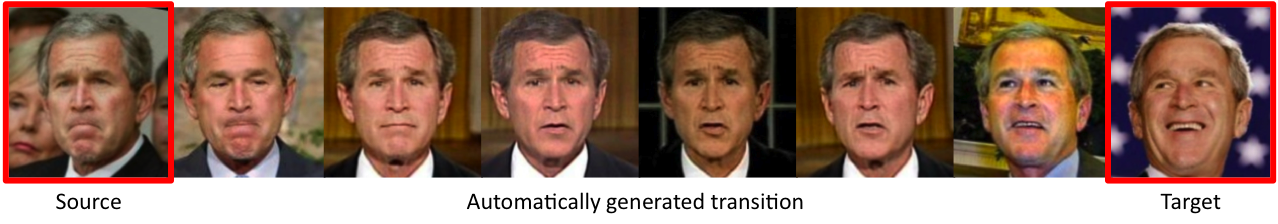
\includegraphics[width=\textwidth]{photobios}

\begin{itemize}
\item These snapshots can be taken from different viewing angles and rotations
\item We must {\em factor out} the relevant symmetries (e.g. translations and rotations) before constructing a representative trajectory
\end{itemize}

\vspace{0.1in}
We will construct a representative trajectory of the developmental~dynamics \\ in a {\em Drosophila} embryo from snapshots of the embryo

\foreach \i in {1, 15, 20, 25, 30, 35, 40, 45, 52} {
	\includegraphics[width=0.1\textwidth]{aligned_\i}
}
\end
{frame}

\begin{frame}{Imaging Dorsoventral Patterns in {\em Drosophila} \footcite{chung2010microfluidic}}

	\centering
    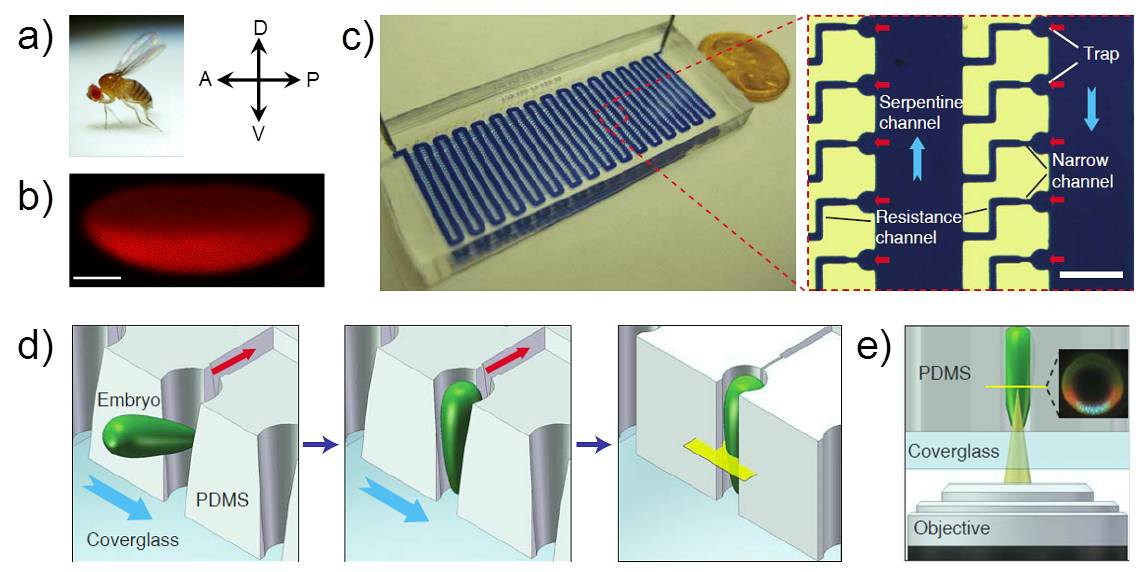
\includegraphics[width=0.75\textwidth]{drosophila_imaging_setup}
    
	\begin{itemize}
        \item We can easily obtain snapshots of many {\em Drosophila} embryos using a high--throughput microfluidic device
        \item Each embryo is fixed at a slightly different developmental time (``cross-sectional data'')
        \item We would like to order the data from multiple embryos in time to reconstruct the developmental dynamics in {\em Drosophila}
    \end{itemize}
\end{frame}


\begin{frame}{ERK Activation in {\em Drosophila}}
	
	\centering
	We would like to reconstruct the spatiotemporal dynamics \\
	of the activation of the ERK pathway in {\em Drosophila} embryos\\
	during nuclear cycle 14 (the third hour of development)

    \centering
	\begin{minipage}{0.3\textwidth}
	    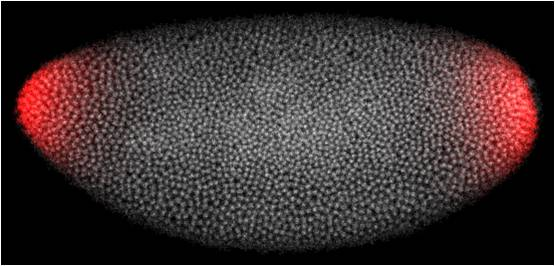
\includegraphics[width=\textwidth]{erk_10min}\\
	    {\scriptsize \em 10 minutes \par}
	\end{minipage}
	\begin{minipage}{0.3\textwidth}
	    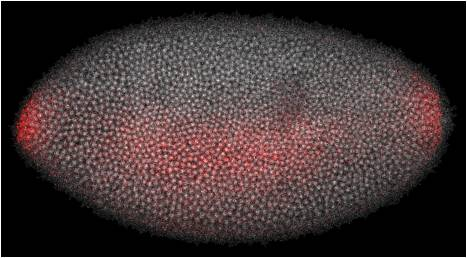
\includegraphics[width=\textwidth]{erk_25min}\\
	    {\scriptsize \em 25 minutes \par}
	\end{minipage}
	\begin{minipage}{0.3\textwidth}
	    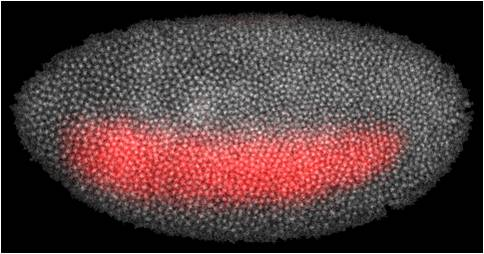
\includegraphics[width=\textwidth]{erk_45min}\\
	    {\scriptsize \em 45 minutes \par}
	\end{minipage}
	
	\begin{itemize}
		\item We measure the activation of ERK by staining embryos for double-phosphorylated ERK (dpERK); ERK is double-phosphorylated  directly downstream of the ERK pathway, and so the presence of dpERK indicates activation of the ERK pathway
	
		\item However, we cannot fluorescently tag ERK within the developing embryo because we are interested in a specific phosphorylation state of the molecule
		
		\item Instead, we must {\em fix} the embryo and then use an antibody stain for dpERK
	
		\item Therefore, we cannot obtain live images of the evolution of dpERK in {\em Drosophila} embryos
	\end{itemize}
	
\end{frame}

%\begin{frame}{Motivation: How Do Cells Obtain Unique Functions?}
%
%    \begin{tikzpicture}
%        \node (embryo1) {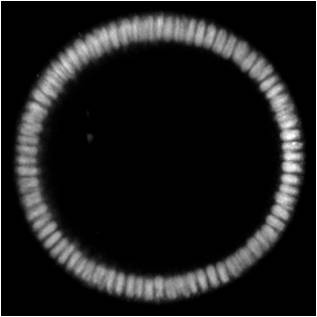
\includegraphics[width=0.15\textwidth]{embryo_bw}};
%        \draw[gray,<->] (embryo1.south west) --  (embryo1.south east) node[below,midway] { \tiny $100 \mu m$};
%        
%        \node[below=0.1in of embryo1, text width=0.15\textwidth, align=center] (text1)  {{\scriptsize Cells}};
%		
%		\node[right=0.3in of embryo1] (embryo3)  {     
%        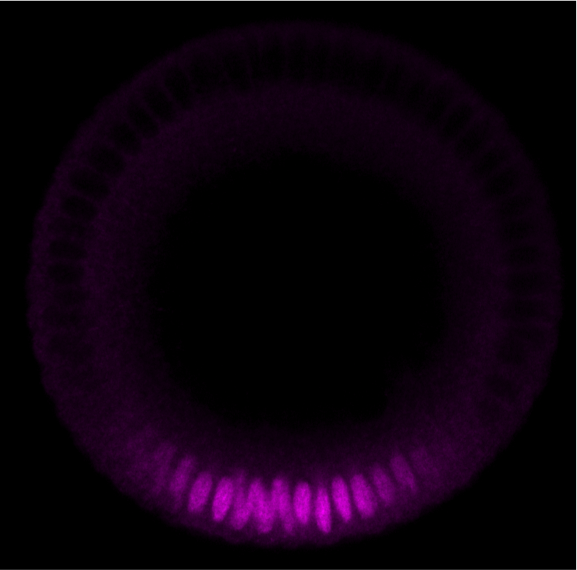
\includegraphics[width=0.2\textwidth]{dorsal}} edge[<-] (embryo1);
%        \draw[gray, <->] (embryo3.south west) --  (embryo3.south east) node[below,midway] { \tiny $100 \mu m$};
%        \node[below=0.1in of embryo3, text width=0.15\textwidth, align=center] (text2)  {{\scriptsize Morphogens diffuse \footnotemark \par}};
%		\node[above=0in of embryo3] (flag)  {     
%        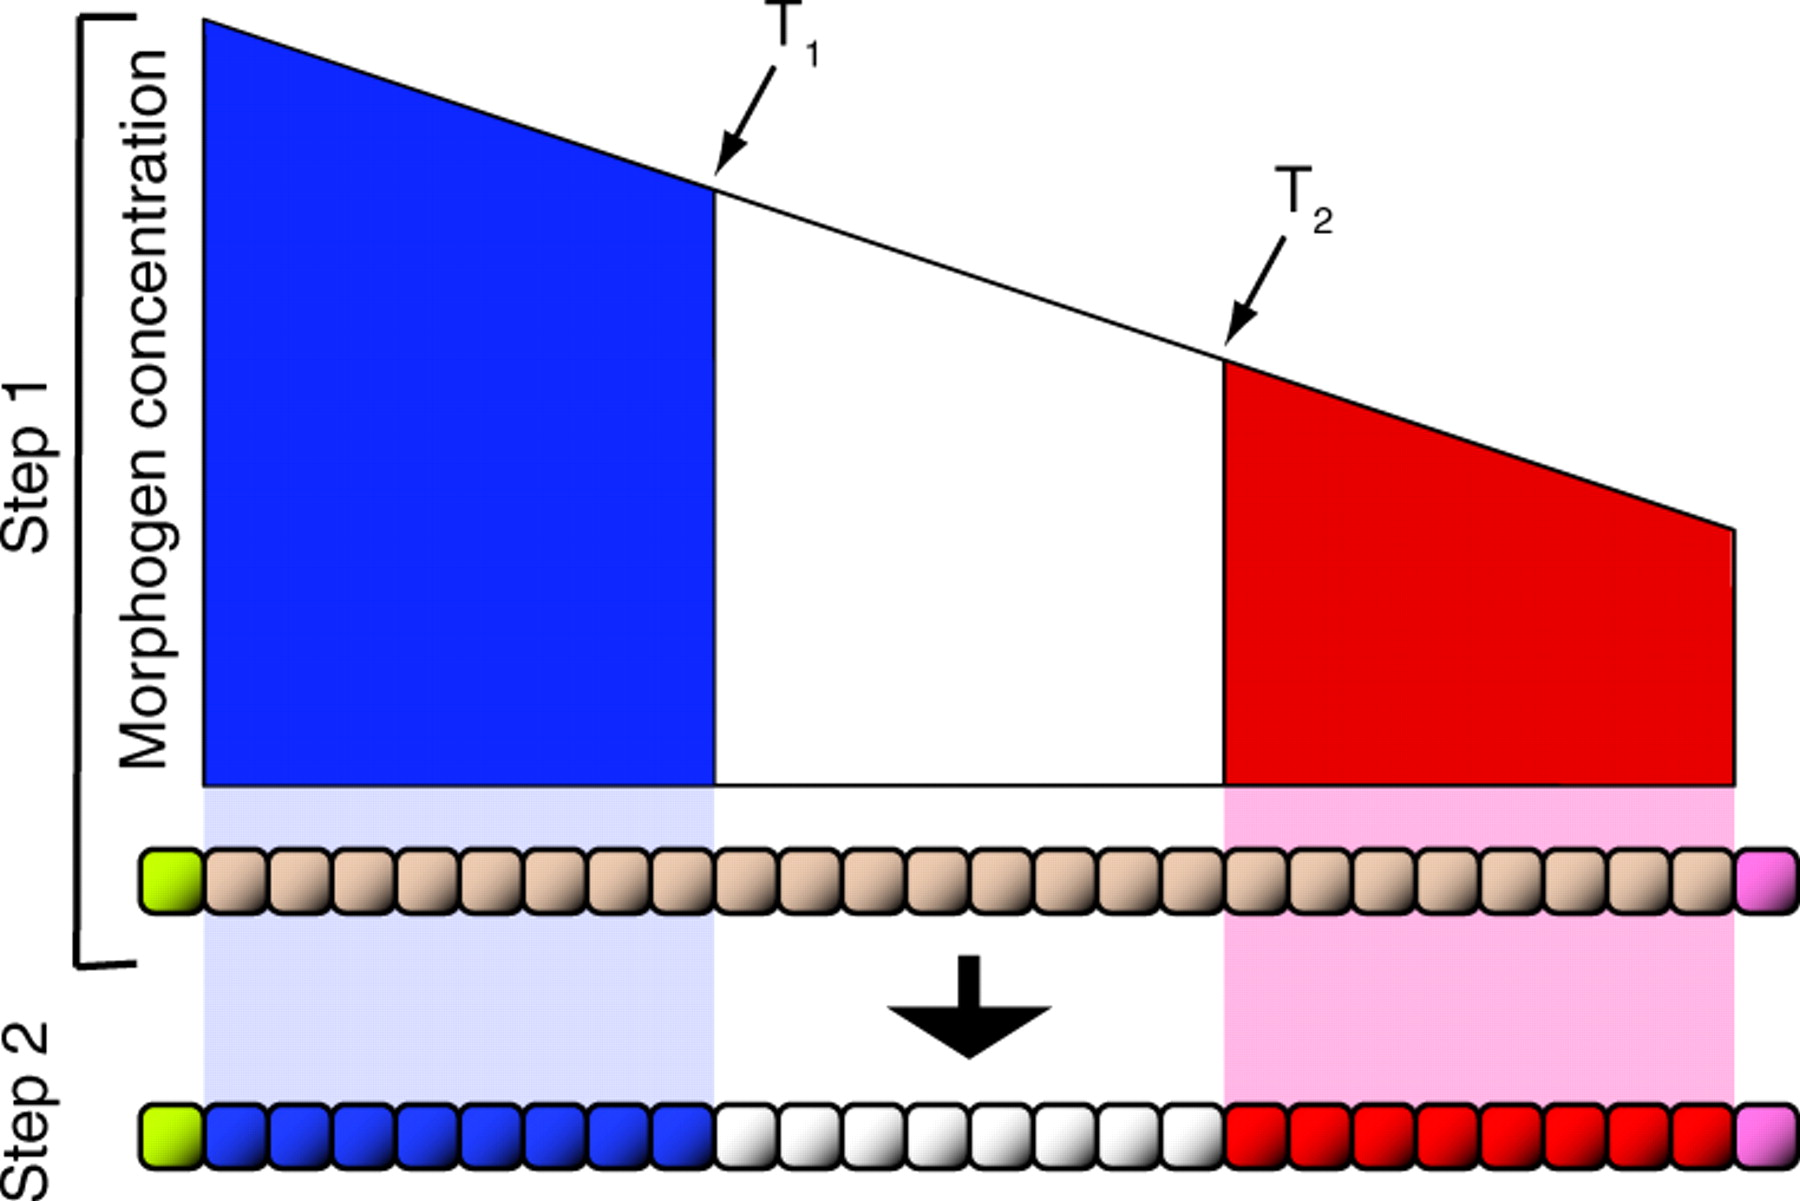
\includegraphics[width=0.2\textwidth]{french_flag}};
%        
%        \node[right=0.3in of embryo3] (embryo2)  {     
%        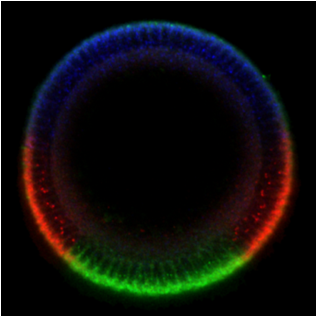
\includegraphics[width=0.15\textwidth]{embryo_color}} edge[<-] (embryo3);
%                \draw[gray,<->] (embryo2.south west) --  (embryo2.south east) node[below,midway] { \tiny $100 \mu m$};
%
%        \node[below=0.1in of embryo2, text width=0.15\textwidth, align=center] (text2)  {{\scriptsize Different proteins are produced in different regions \par}};
%
%        \node[right=0.3in of embryo2] (nervous)  {
\includegraphics[width=0.15\textwidth]{nervous_system}} edge[<-] (embryo2);
%
%        \node[above=0.1in of nervous] (skin)  {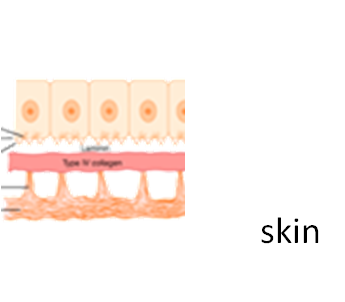
\includegraphics[width=0.15\textwidth]{skin}} edge[<-] (embryo2);
%
%        \node[below=0.1in of nervous] (muscle)  {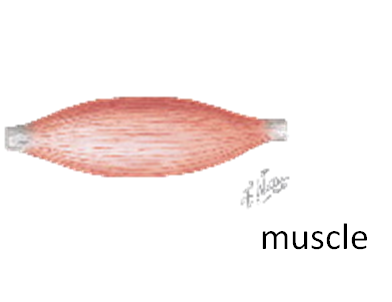
\includegraphics[width=0.15\textwidth]{muscle}} edge[<-] (embryo2);
%    \end{tikzpicture}
%
%	\footcitetext{jaeger2008regulative}
%	
%	{\small Different pathways are {\em activated} in different areas of the organism,  
%	leading to the production of different proteins and different cells developing~different~functions \par}
%
%\end{frame}
%
%\begin{frame}{ERK Activation Across Species}
%	\begin{itemize}
%		\item 	Extracellular signal-regulated kinases (ERKs) are singalling proteins that regulate mitosis and meiosis in cells.
%
%		\item	ERK activation is conserved among many species.
%
%	\end{itemize}
%	
%    \centering
%    \begin{minipage}{0.2\textwidth}
%        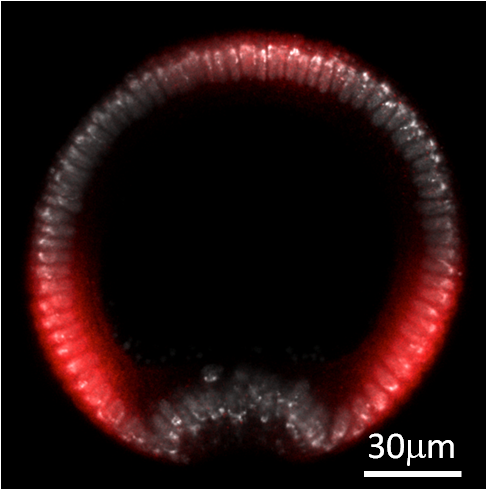
\includegraphics[width=\textwidth]{drosophila_erk}\\
%        {\scriptsize \em Drosophila \par}
%    \end{minipage}
%    \hspace{0.5in}
%    \begin{minipage}{0.2\textwidth}
%        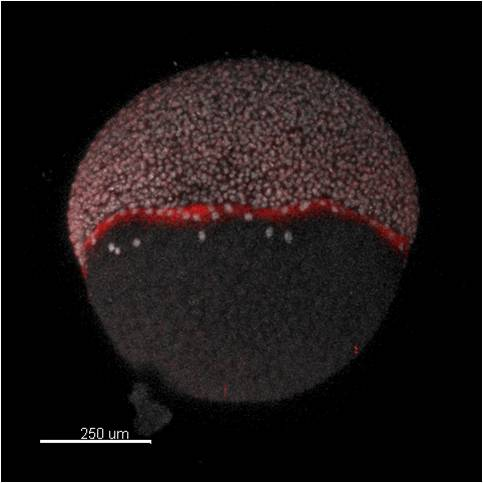
\includegraphics[width=\textwidth]{zebrafish_erk}\\
%        {\scriptsize \em zebrafish \par}
%    \end{minipage}
%    \vspace{0.2in}
%    
%    \centering
%    \begin{minipage}{0.4\textwidth}
%        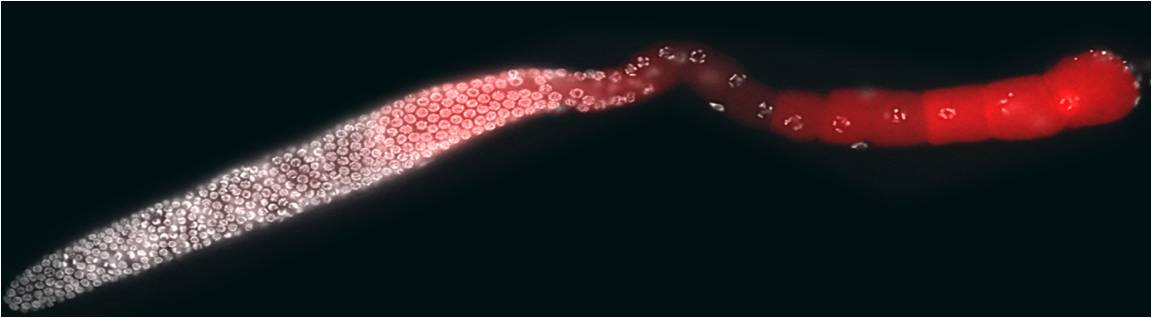
\includegraphics[width=\textwidth]{celegans_erk}\\
%        {\scriptsize \em C. elegans \par}
%    \end{minipage}
%    
%	\vspace{0.1in}
%    ERK stained (in red) in several model organisms.
%    
%\end{frame}

\begin{frame}{Measuring Developmental Time from Membrane Markers}

	\centering
    The current standard practice is to use membrane thickness \\to measure the age of an embryo \footcite{lim2013kinetics, lecuit2002slam}\\
    \vspace{0.1in}
    \begin{tikzpicture}
        \node (dpERK_5min) {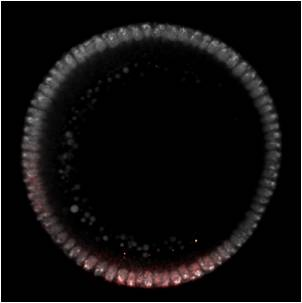
\includegraphics[width=0.1\textwidth]{dpERK_5min}};
        \node[right=0in of dpERK_5min] (mem_5min) {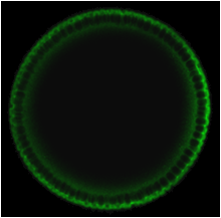
\includegraphics[width=0.1\textwidth]{membrane_5min}};
        \node[below=0.1in of dpERK_5min] (dpERK_20min) {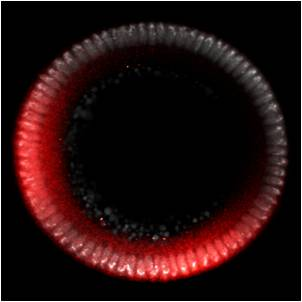
\includegraphics[width=0.1\textwidth]{dpERK_20min}};
        \node[right=0in of dpERK_20min] (mem_20min) {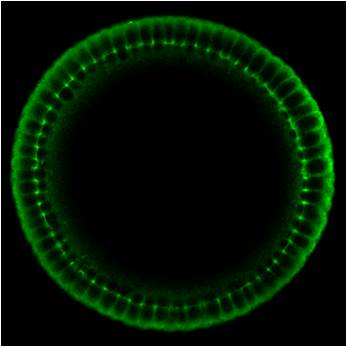
\includegraphics[width=0.1\textwidth]{membrane_20min}};
        \node[below=0.1in of dpERK_20min] (dpERK_45min) {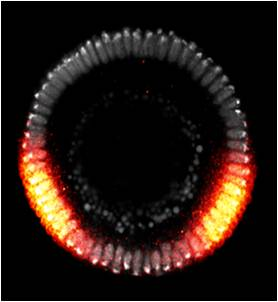
\includegraphics[width=0.1\textwidth]{dpERK_45min}};
        \node[right=0in of dpERK_45min] (mem_45min) {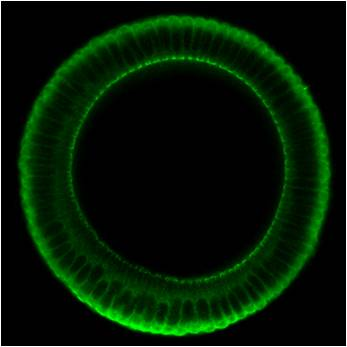
\includegraphics[width=0.1\textwidth]{membrane_45min}};
        \node[below=0.25in of $(dpERK_45min)!0.5!(mem_45min)$, text width=0.3\textwidth, align=center](text1) {{\small \em We stain each embryo for dpERK and membrane proteins \par}};
        \node[right=0.5in of mem_20min] (calibration) {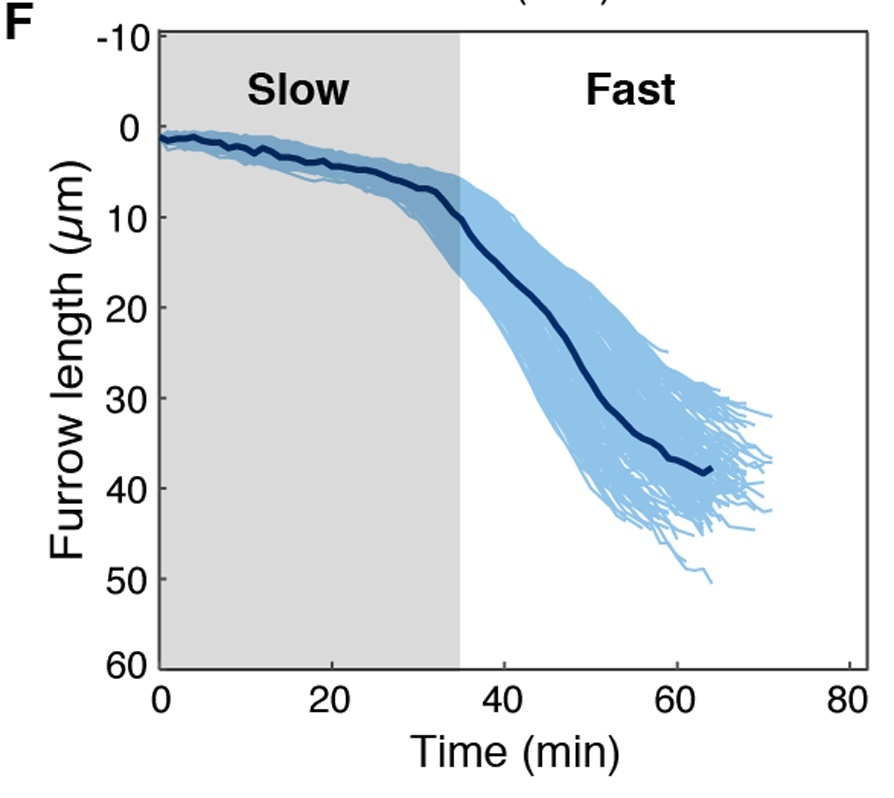
\includegraphics[width=0.3\textwidth]{calibration_curve}} edge[<-] (mem_5min) edge[<-] (mem_20min) edge[<-] (mem_45min);
        \node[below=0in of calibration, text width=0.3\textwidth, align=center](text2) {{\small \em The membrane thickness or ``furrow length'' is monotonic in time or age of the embryo \par}};
        \node[right=2.5in of mem_20min] (time_20) {20 minutes} edge[<-] (calibration);
        \node[right=2.5in of mem_5min] (time_5) {5 minutes} edge[<-] (calibration);
        \node[right=2.5in of mem_45min] (time_45) {45 minutes} edge[<-] (calibration);
        \node[below=0in of time_45, text width=0.25\textwidth, align=center](text2) {{\small \em We can calculate the age of each embryo from the membrane thickness \par}};
    \end{tikzpicture}

\end{frame}

\begin{frame}{Reconstructing Dynamics from Snapshots}

	\begin{tikzpicture}
		\node (schematic) {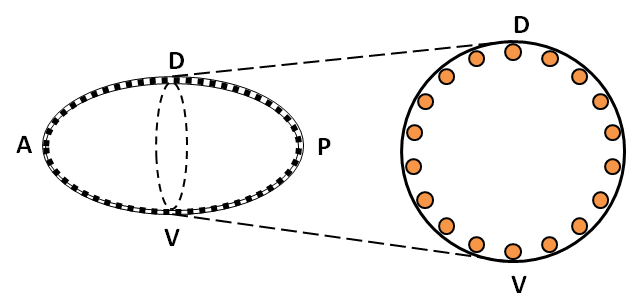
\includegraphics[width=0.25\textwidth]{drosophila_schematic}};
		\node [below=0in of schematic, text width=0.2\textwidth, align=center] (text1) {{\scriptsize Schematic of {\em Drosophila} embryo \\ (longitudinal and cross-section) \par}};

		\node [right=0.2in of schematic] (dpERK_image) {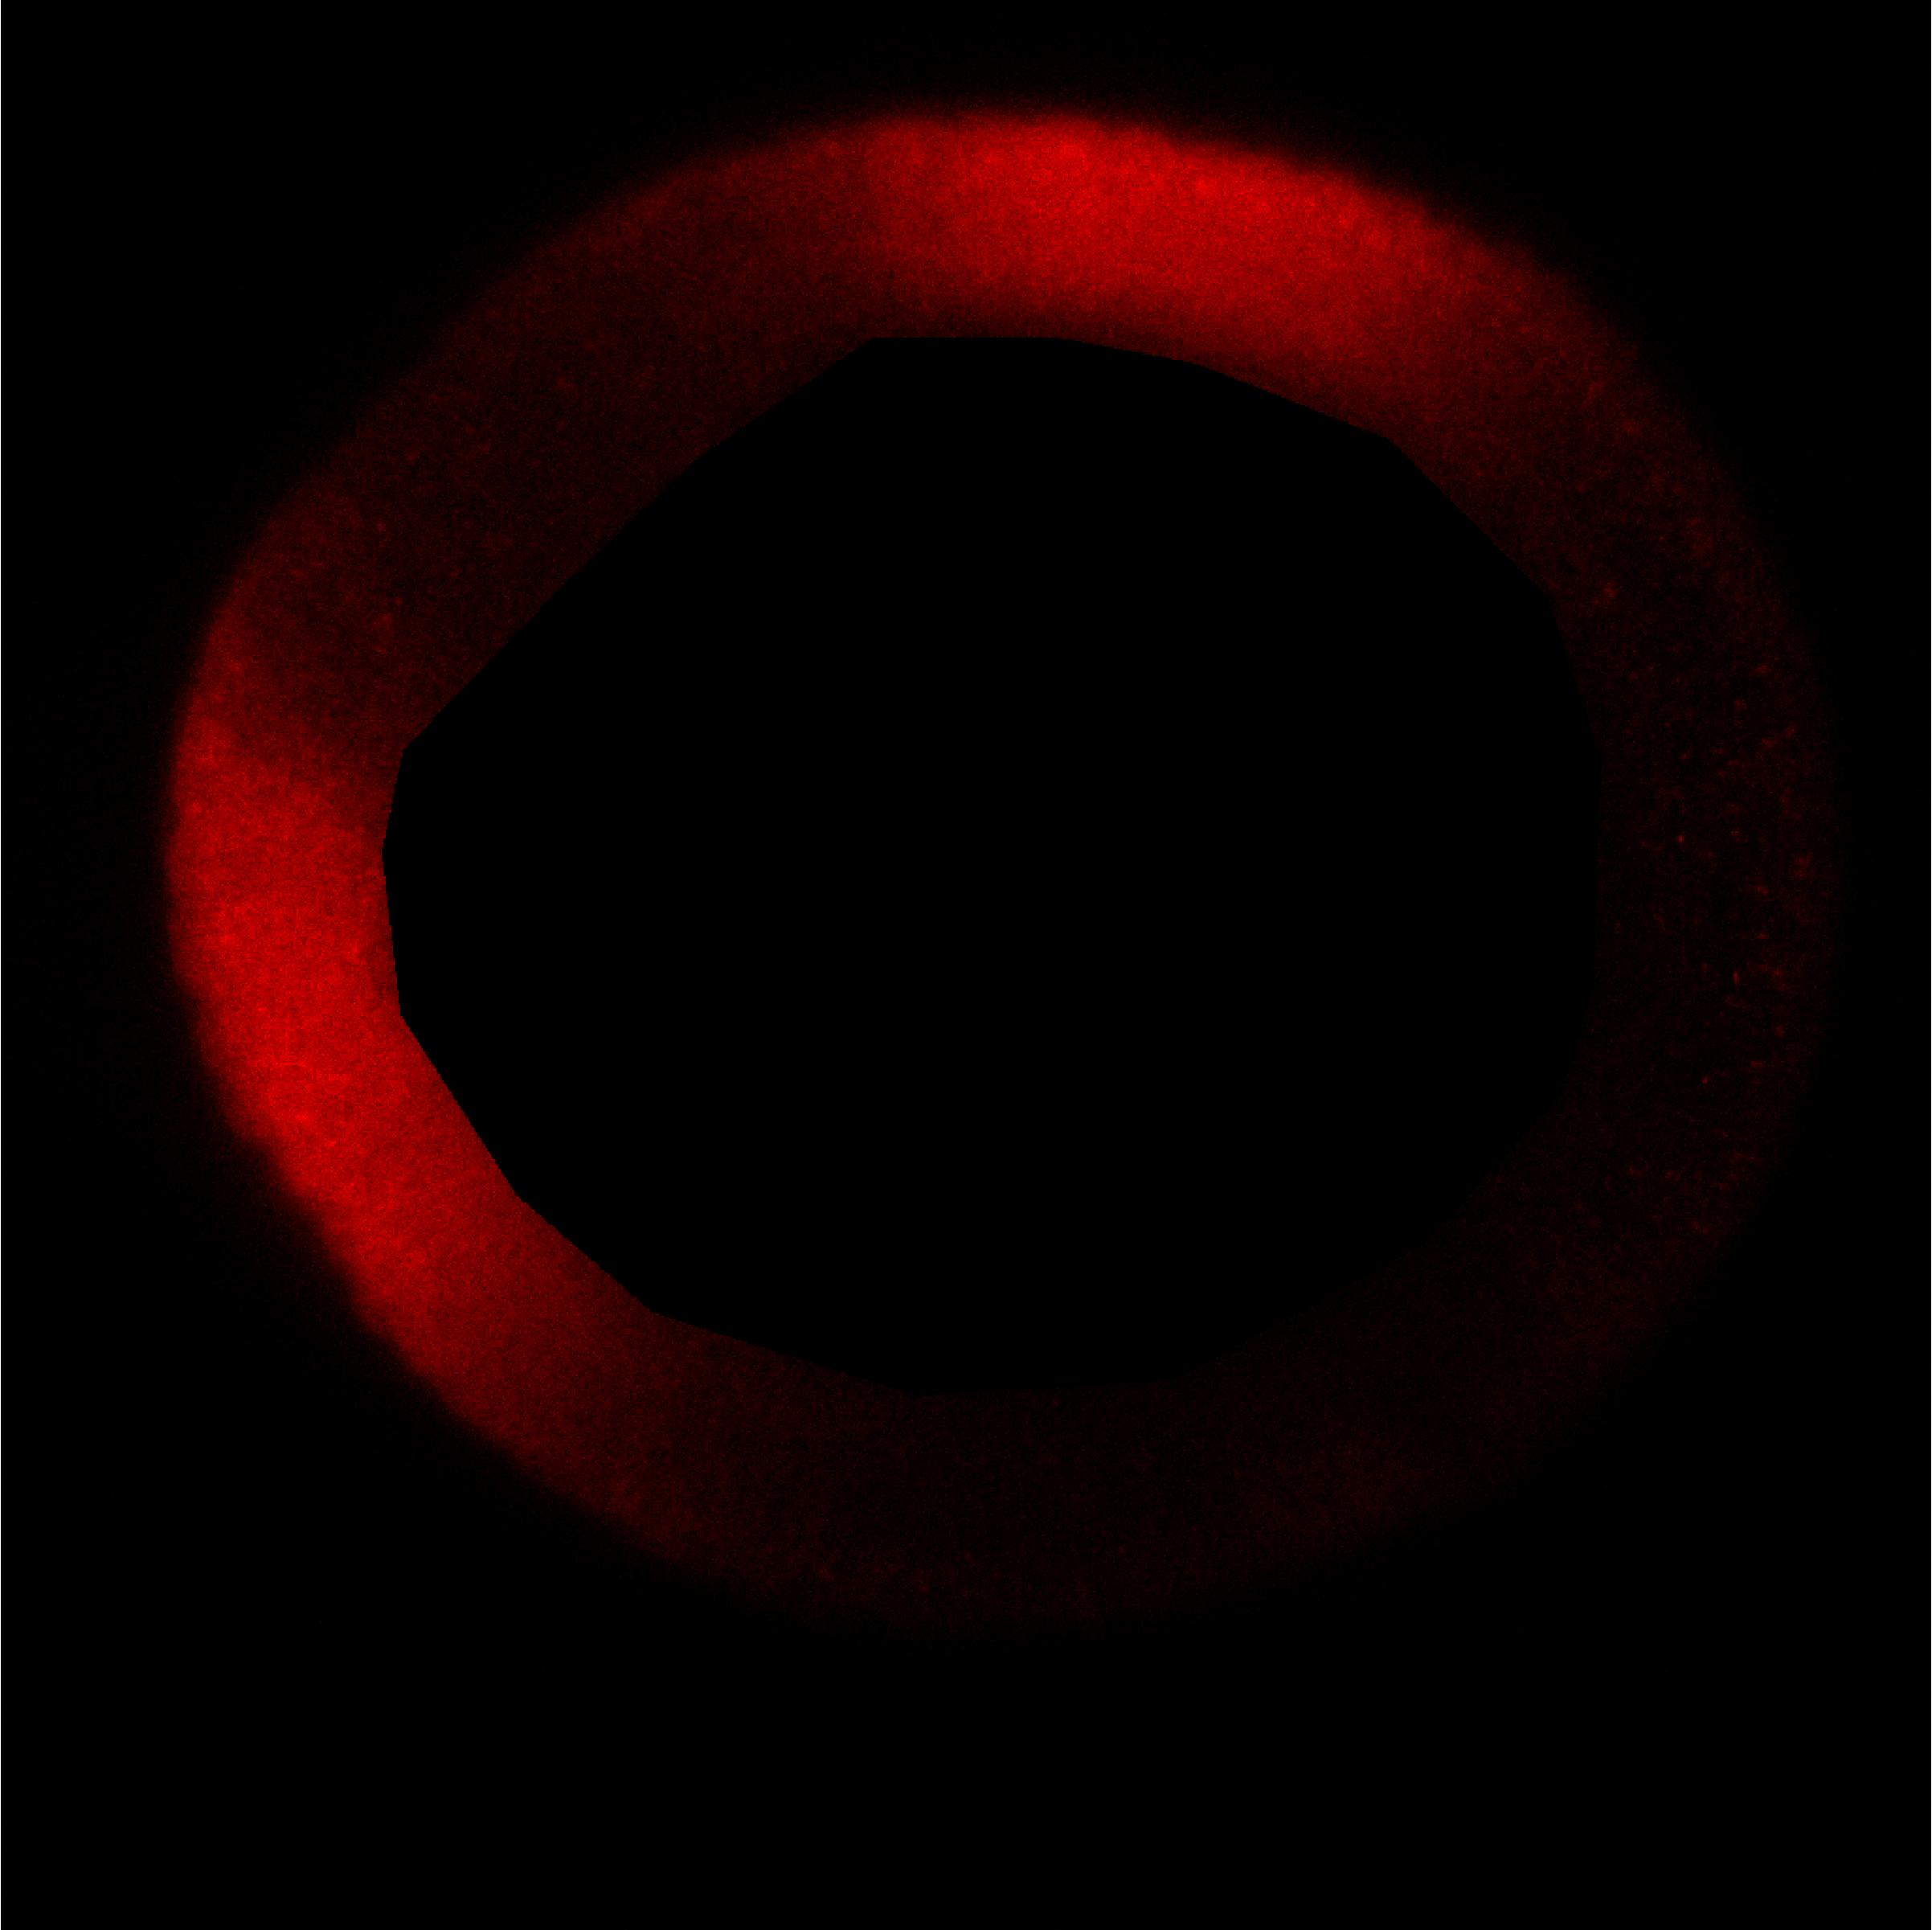
\includegraphics[width=0.15\textwidth]{drosophila_dpERK}} edge[<-] (schematic);
		\draw[gray,<->] (dpERK_image.south west) --  (dpERK_image.south east) node[below,midway] { \tiny $100 \mu m$};
		\node [below=0.1in of dpERK_image, text width=0.2\textwidth, align=center] (text1) {{\scriptsize Embryo cross-section fluorescently stained for the protein dpERK \par}};
		
		\node [right=0.2in of dpERK_image] (dpERK_circle) {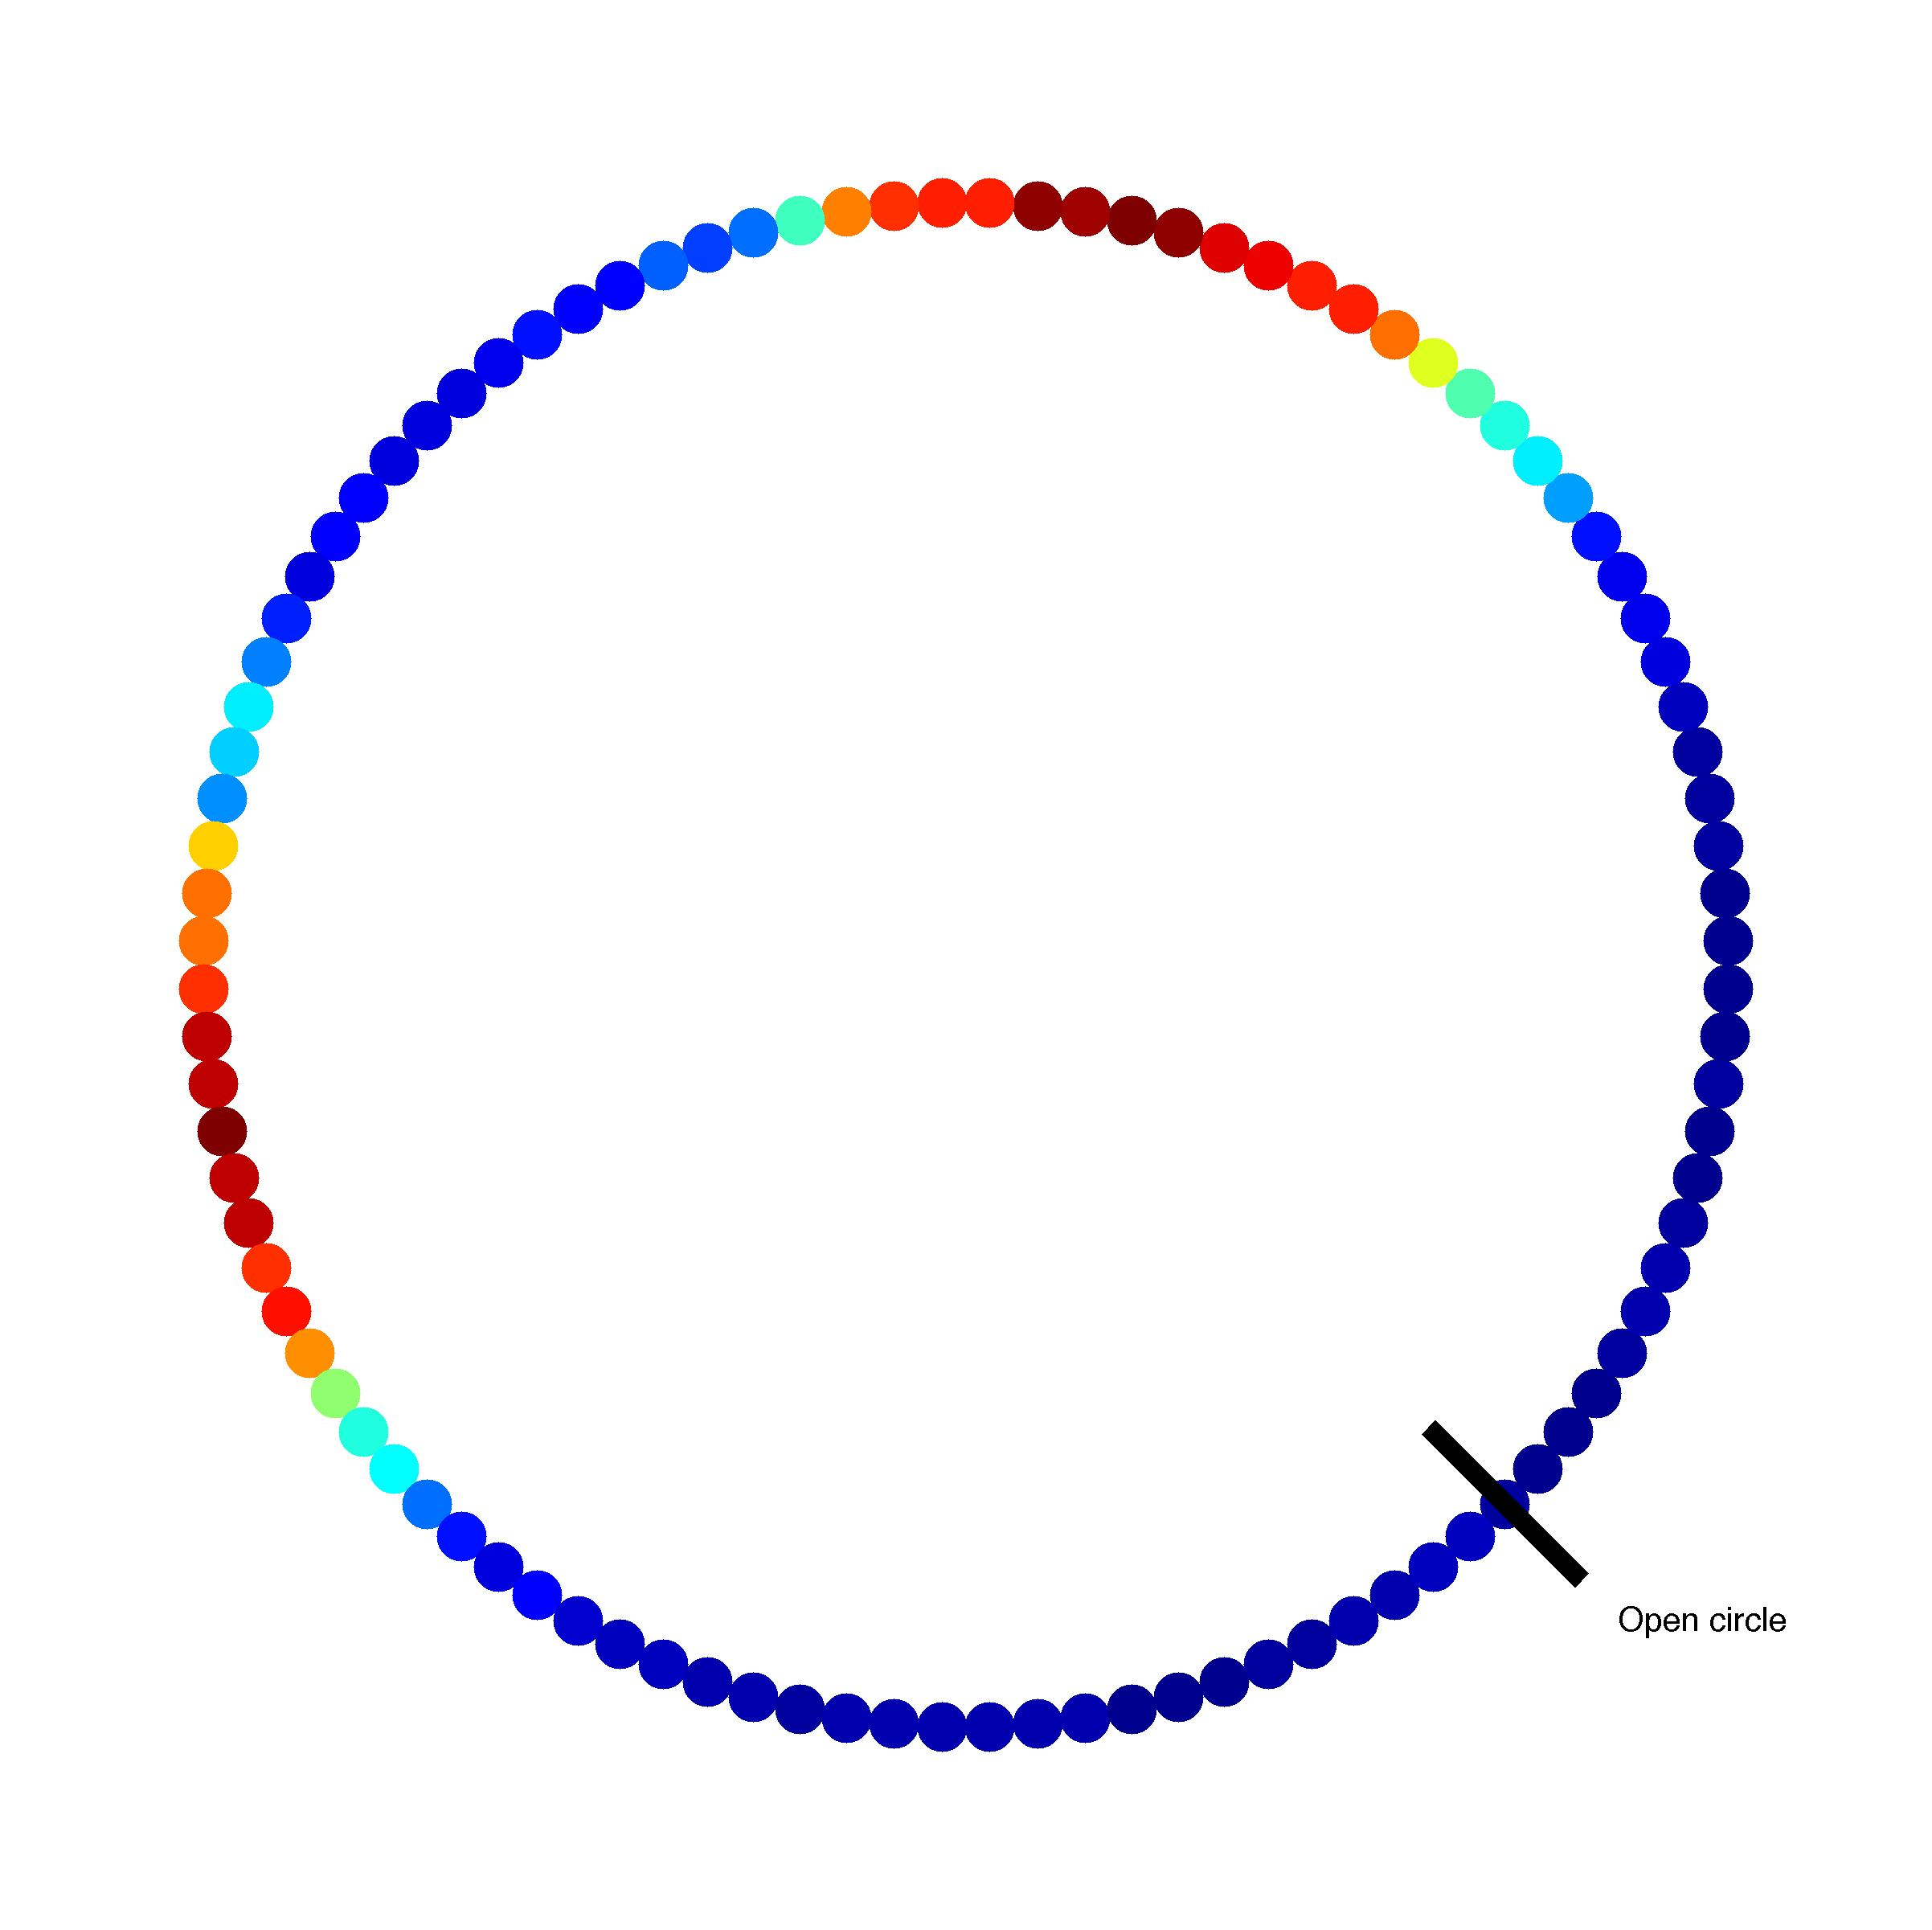
\includegraphics[width=0.15\textwidth]{circle_profile.jpg}} edge[<-] (dpERK_image);
		\node [below=0in of dpERK_circle, text width=0.2\textwidth, align=center] (text1) {{\scriptsize Fluorescent staining is converted to intensity of dpERK around the circumference of the embryo \par}};
		
		\node [right=0.2in of dpERK_circle] (dpERK_line) {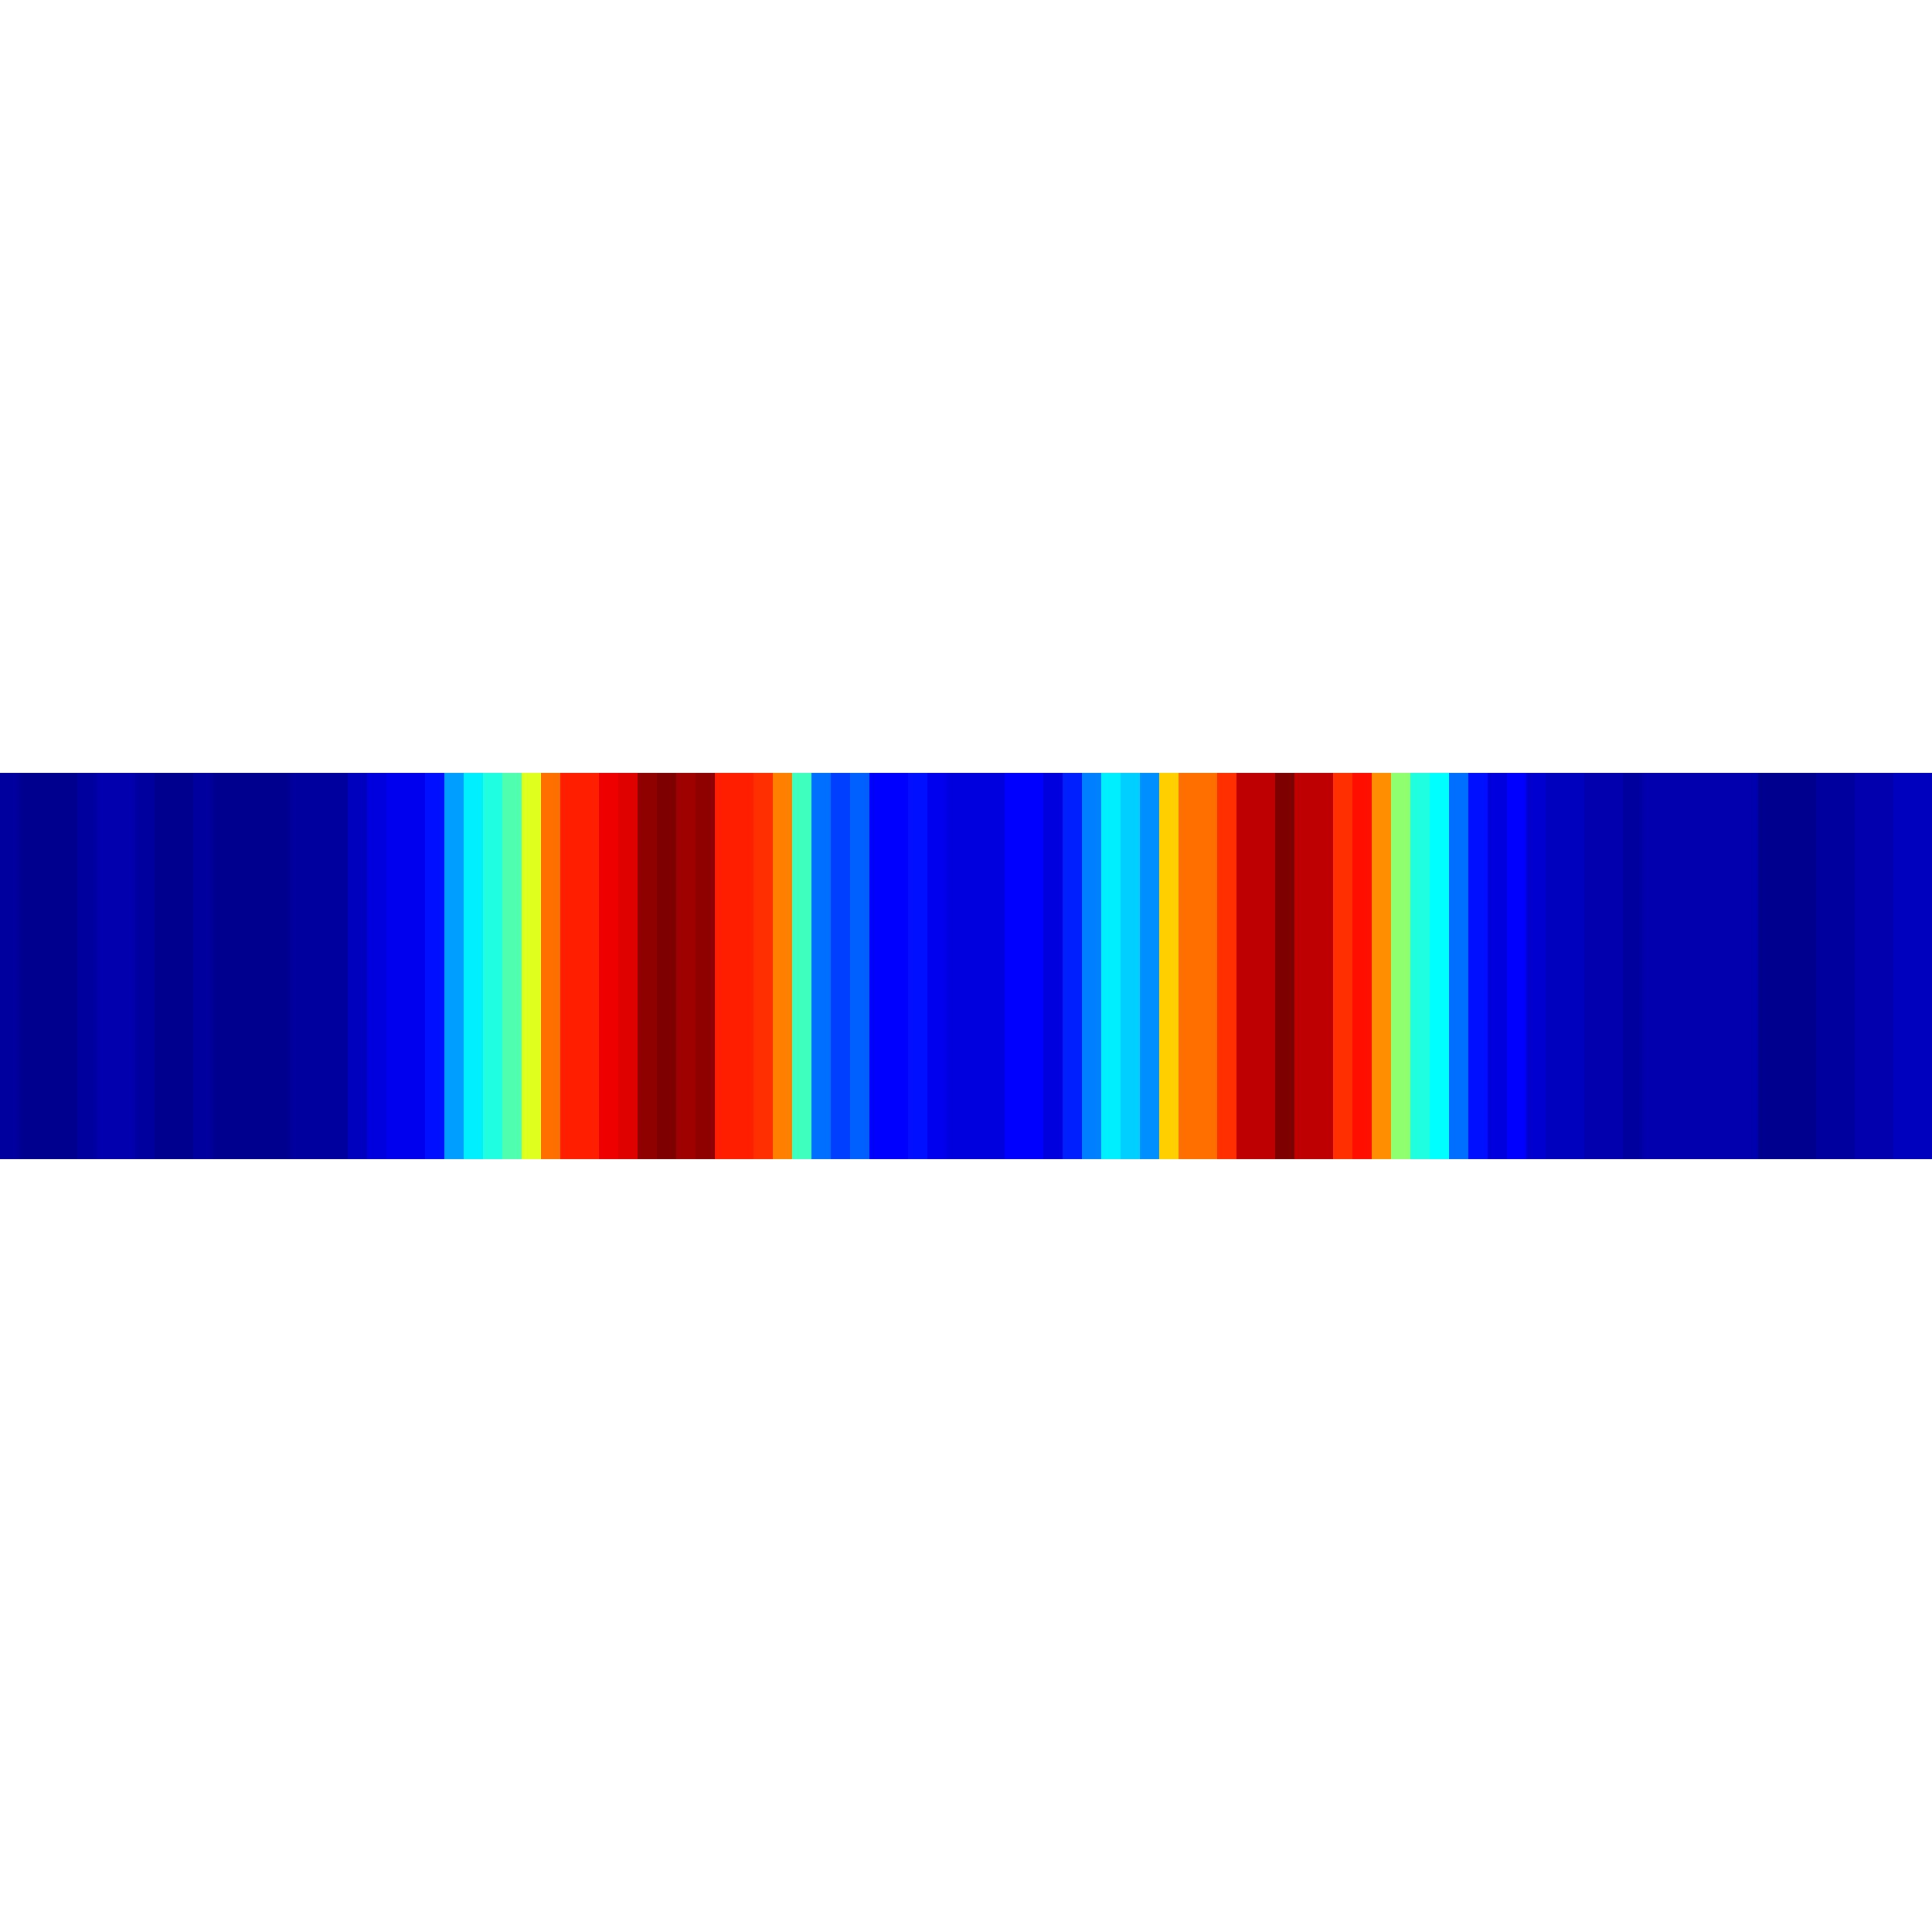
\includegraphics[width=0.2\textwidth, height=0.1in]{line_profile.jpg}} edge[<-] (dpERK_circle);
		\node [below=0in of dpERK_line, text width=0.2\textwidth, align=center] (text1) {{\scriptsize The circumference of the embryo is ``unrolled'' to form an intensity profile for the embryo on a line \par}};
		
	\end{tikzpicture}
	
	\centering
    \begin{tikzpicture}
        \node (fig1) {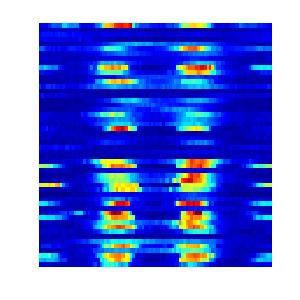
\includegraphics[width=0.35\textwidth]{data_unordered}};
        \node[right of=fig1, node distance=0.55\textwidth] (fig2) {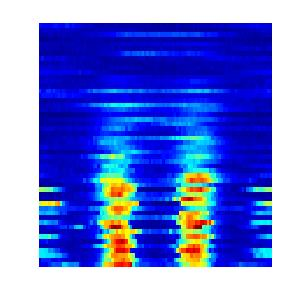
\includegraphics[width=0.35\textwidth]{data_ordered_membrane}};
        \draw [->] (fig1.east) -- (fig2.west) node[above,midway] {\tiny Order using membrane thickness};
    \end{tikzpicture}
	
	We would like to order the snapshots {\em without} measuring the membrane thickness.
	
\end{frame}


\section[Concentration Profiles and Principal Component Analysis]{Temporally Ordering Pre-Aligned Concentration Profiles Using~Principal~Component~Analysis}

\begin{frame}{Principal Component Analysis for Ordering Data}

    \begin{columns}[T]
        \begin{column}{0.3 \textwidth}
            \includegraphics[width=0.8\textwidth]{../Stas_data/group_meeting_5Feb2013/example1_all}

            {\scriptsize This data is similar to the {\em Drosphila} data; it is clearly ordered in time \par}
        \end{column}

        \begin{column}{0.3 \textwidth}
            \includegraphics[width=0.8\textwidth]{../Stas_data/group_meeting_5Feb2013/example1_coarse}

            {\scriptsize We can look at a ``coarsened'' representation of the data with only three spatial components \par}
        \end{column}

        \begin{column}{0.3 \textwidth}
            \includegraphics[width=0.8\textwidth]{../Stas_data/group_meeting_5Feb2013/example1_embedding}

            {\scriptsize If we plot the three-dimensional data and color them in time, we see they fall on a line and are correlated along this line in time \par}
        \end{column}
    \end{columns}
    %\vspace{0.1 in}

	\begin{columns}
	\begin{column}{0.7\textwidth}
	\begin{itemize}
	{\small   
   \item If we embedded the original (high-dimensional) data, the data would fall on a line in high-dimensional space

   \item We assume that the data is ordered in time when projected along this line
   
   \item We would like an automatic way to find this line in higher dimensions
      
  \item Principal Component Analysis (PCA) \footnotemark finds this line by calculating the direction(s) of maximum variance %in a data set
  \par}
  \end{itemize}
  \end{column}
  \begin{column}{0.25\textwidth}
  \begin{block}{{\small PCA Algorithm}}
 {\footnotesize
  	Calculate covaraince matrix
  	$$C =X^T X$$	
  	Compute eigenvectors and eignevalues
  	$$C V = V \Lambda$$
  	$V$ are the principal components
  %\end{block}
  \par}
  \end{block}
  \end{column}
  \end{columns}
  
  \footcitetext{shlens2005tutorial}
\end{frame}

%\begin{frame}{PCA: Covariance Matrix}
%  \begin{itemize}
%  \item We have $n$ {\bf data points}, each in $d$ dimensions, denoted $x_1, x_2, \dots, x_n \in \mathbb{R}^d$, where $x_{i,j}$ denotes the $j^{th}$ component of data point $i$
%  \item We first define the {\bf mean-centered} data points $\hat{x}_i$ as $$\hat{x}_{i,j} = x_{i,j} - \frac{1}{n} \sum_{i=1}^{n} x_{i,j}$$
%  \item Let $X \in \mathbb{R}^{n \times d}$ denote the data matrix, where the $i^{th}$ row of $X$ contains $\hat{x}_i$
%  \item The {\bf covariance matrix} $R \in \mathbb{R}^{d \times d}$ can be estimated as $$R = \frac{1}{n-1} X^T X$$
%  \end{itemize}
%\end{frame}
%
%\begin{frame}{PCA: Eigendecomposition}
%\begin{columns}
%\begin{column}{0.7\textwidth}
%  \begin{itemize}
%    \item We then compute the {\bf eigenvectors} $v_1, v_2, \dots, v_d$ and {\bf eigenvalues} $\lambda_1, \lambda_2, \dots, \lambda_d$ of $R$ (all eigenvectors are normalized to 1)
%    \item By construction, $R$ is symmetric and positive semi-definite and is therefore guaranteed to have real non-negative eigenvalues and orthogonal real eigenvectors
%    \item We {\bf order} the eigenvector/eigenvalue pairs such that $\lambda_1 \ge \lambda_2 \ge \dots \ge \lambda_d$
%    \item $v_1, v_2, \dots, v_d$ are called the {\bf principal components}, and $\lambda_j$ measures the {\bf variance} captured by principal component $j$
%  \end{itemize}
%  \end{column}
%
%  \begin{column}{0.3\textwidth}
%        \includegraphics[width=\textwidth]{../Stas_data/group_meeting_5Feb2013/PCA_spectrum1.jpg}\\
%        {\tiny The PCA eigenvalue spectrum; each eigenvalue measures the energy captured by the corresponding eigenvector \par}
%
%        \vspace{0.3 in}
%
%        \includegraphics[width=\textwidth]{../Stas_data/group_meeting_5Feb2013/PCA_mode1.jpg}\\
%        {\tiny The first principal component \par}
%
%  \end{column}
%  \end{columns}
%\end{frame}
%
%\begin{frame}{PCA: Ordering and Projections}
%    \begin{itemize}
%        \item We can calculate the projection of data point $i$ onto principal component $j$ as $a_{i,j} = \langle \hat{x}_i, v_j \rangle = \sum_{k=1}^{d} \hat{x}_{i,k} v_{j,k}$
%        \item $a_{i,j}$ can be viewed as a measure of how much principal component $j$ is represented in data point $i$
%        \item We can order the data by $a_{i,1}$
%        \item Each principal component defines an important ``direction'' in our data; we can compare data sets by comparing their principal components
%    \end{itemize}
%
%    \centering
%    \includegraphics[height=0.3\textheight]{../Stas_data/group_meeting_5Feb2013/data1_scrambled.jpg}
%    \includegraphics[height=0.3\textheight]{../Stas_data/group_meeting_5Feb2013/coeff_scrambled.jpg}\\
%    {\Tiny The scrambled data (left) and the projection coefficient for each data point onto the first principal component (right).\\
%    We will sort the data by the values of the projection coefficients. \par}
%
%\end{frame}

\begin{frame}{Ordering {\em Drosophila} Data using PCA}

	\centering
	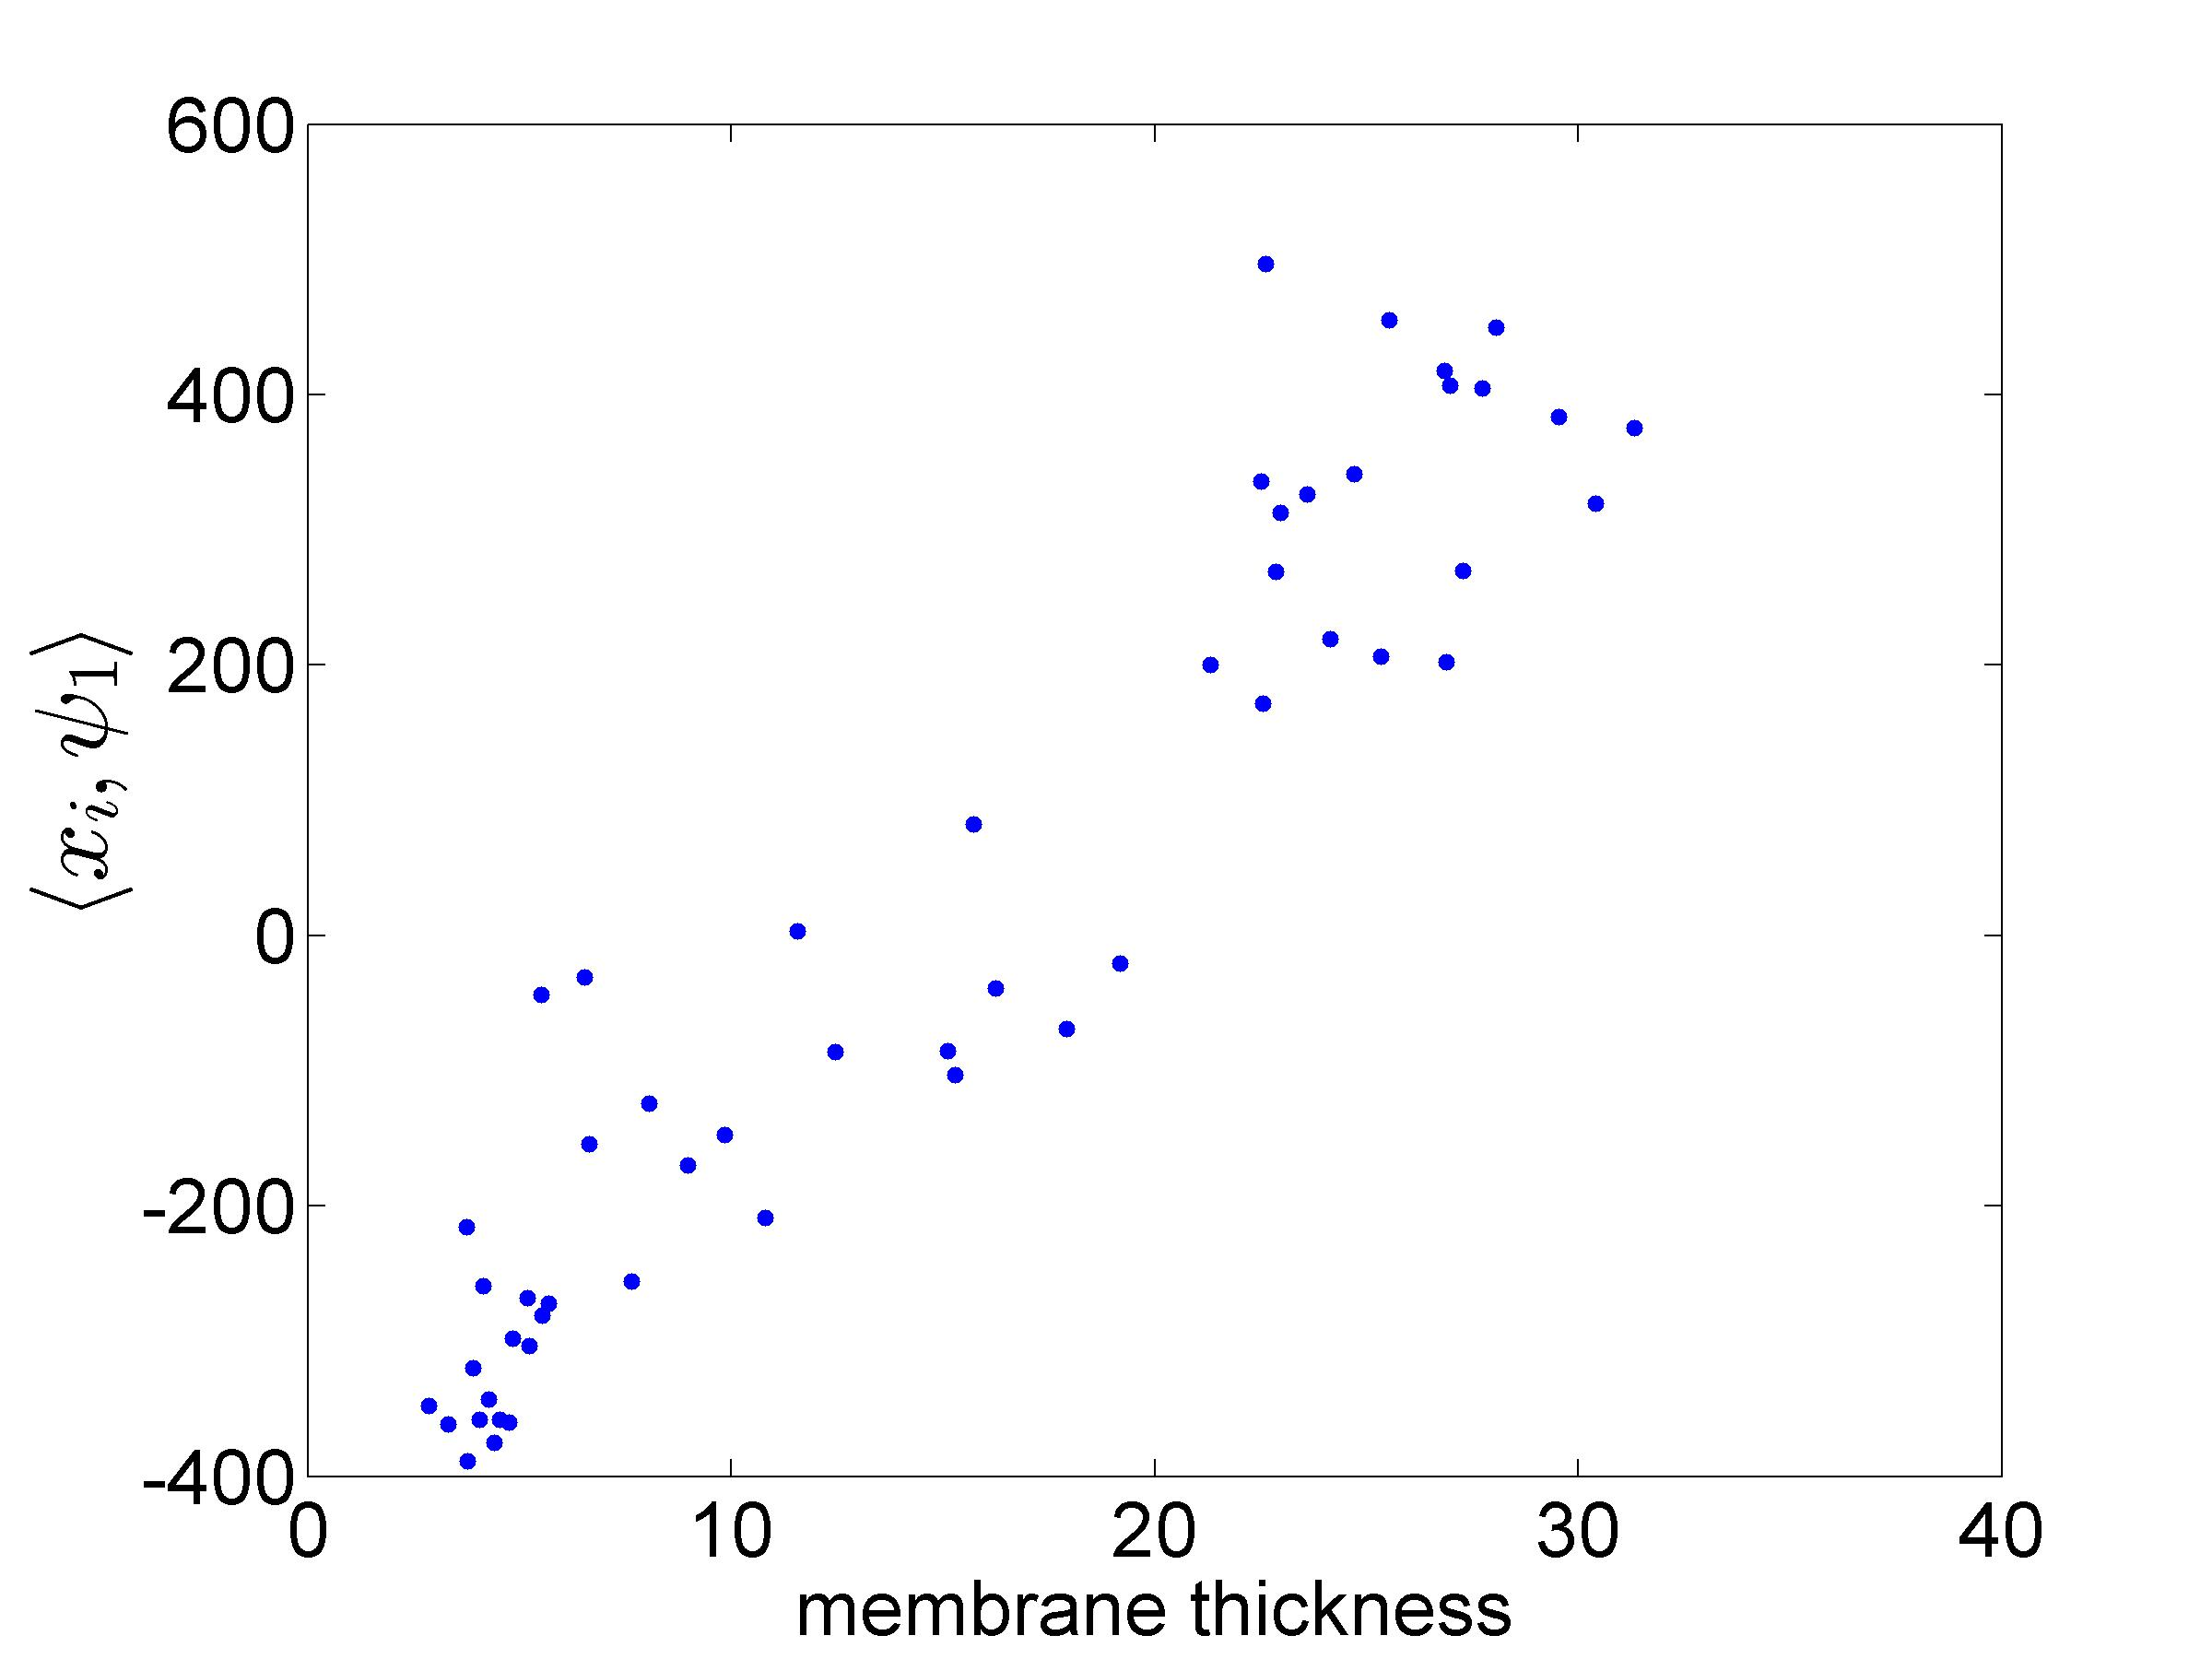
\includegraphics[width=0.3\textwidth]{PCA_time_corr}	
  
  \centering
  \begin{tikzpicture}
  	\node (unordered) {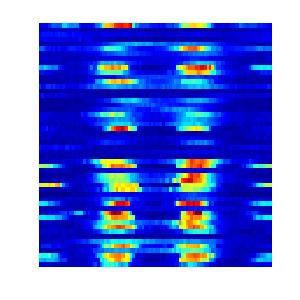
\includegraphics[width=0.3\textwidth]{data_unordered}};
  	\node[right of=unordered, node distance=0.5\textwidth] (ordered) {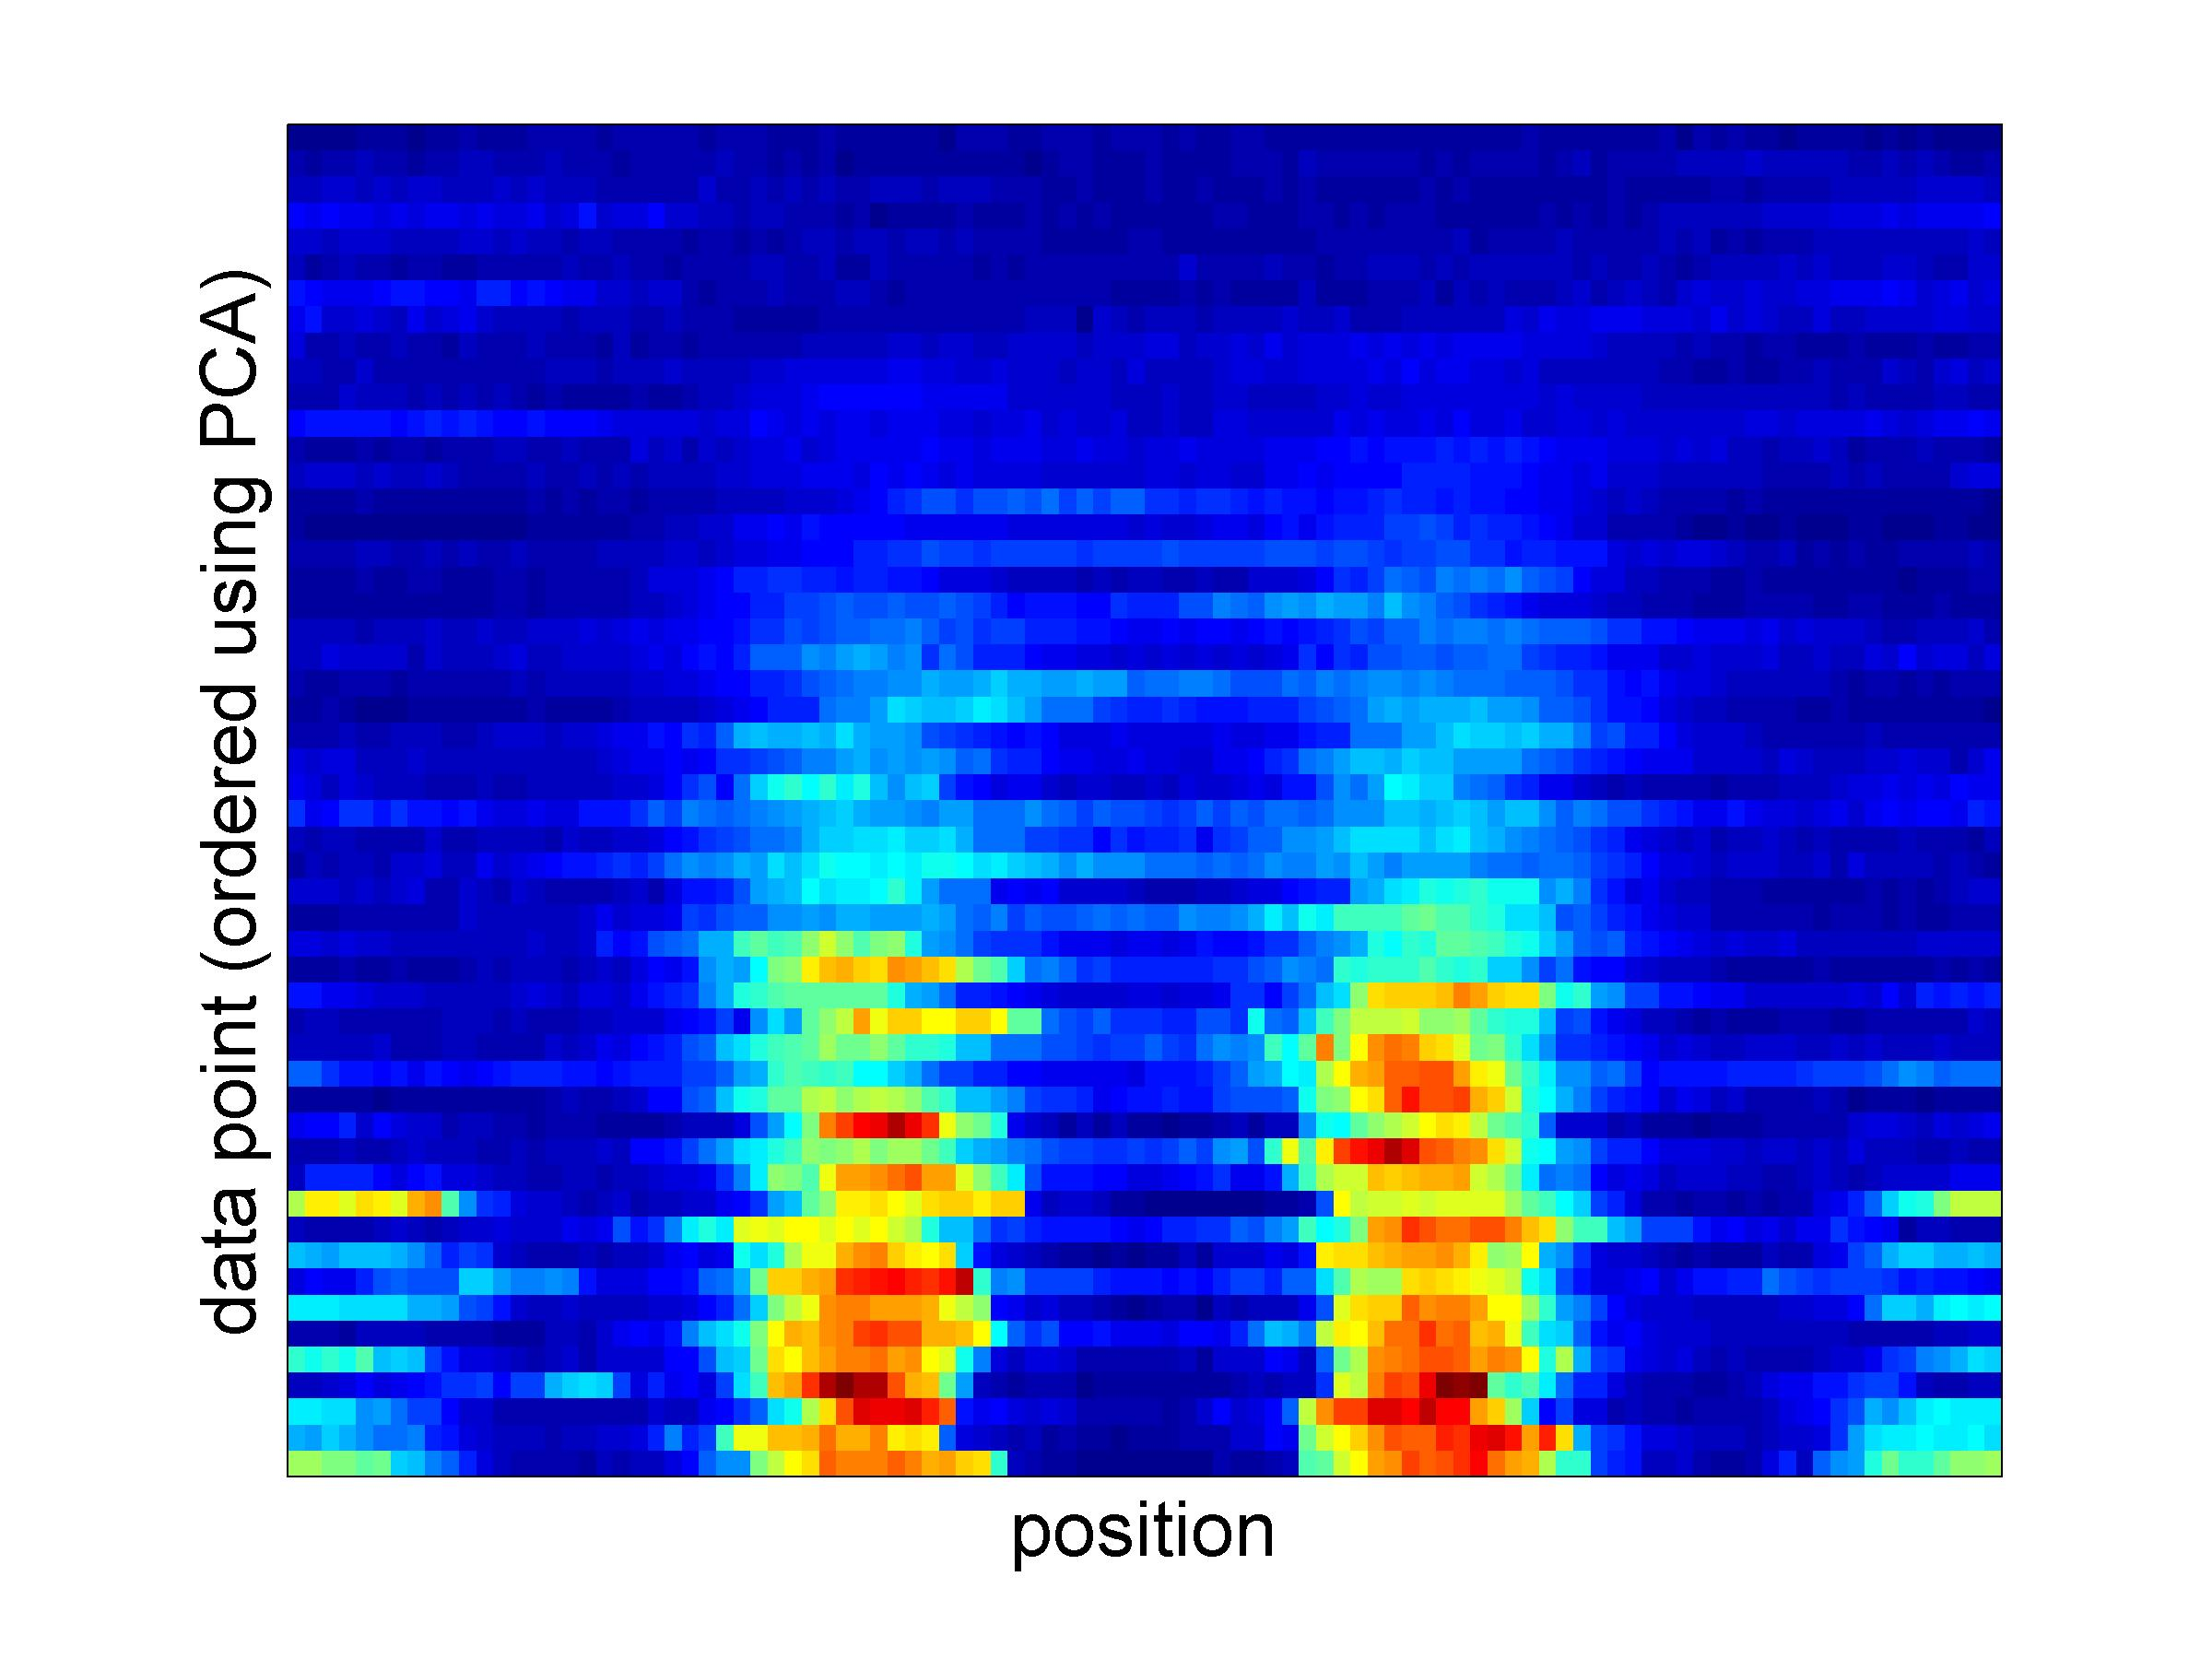
\includegraphics[width=0.3\textwidth]{data_ordered_PCA}};
    \draw [->] (unordered.east) -- (ordered.west);    
  \end{tikzpicture}
  
	
	
\end{frame}


\begin{frame}{Some Problems with PCA}
    \centering
    \begin{tikzpicture}
    	\node[anchor=south west] (PCA_fig) {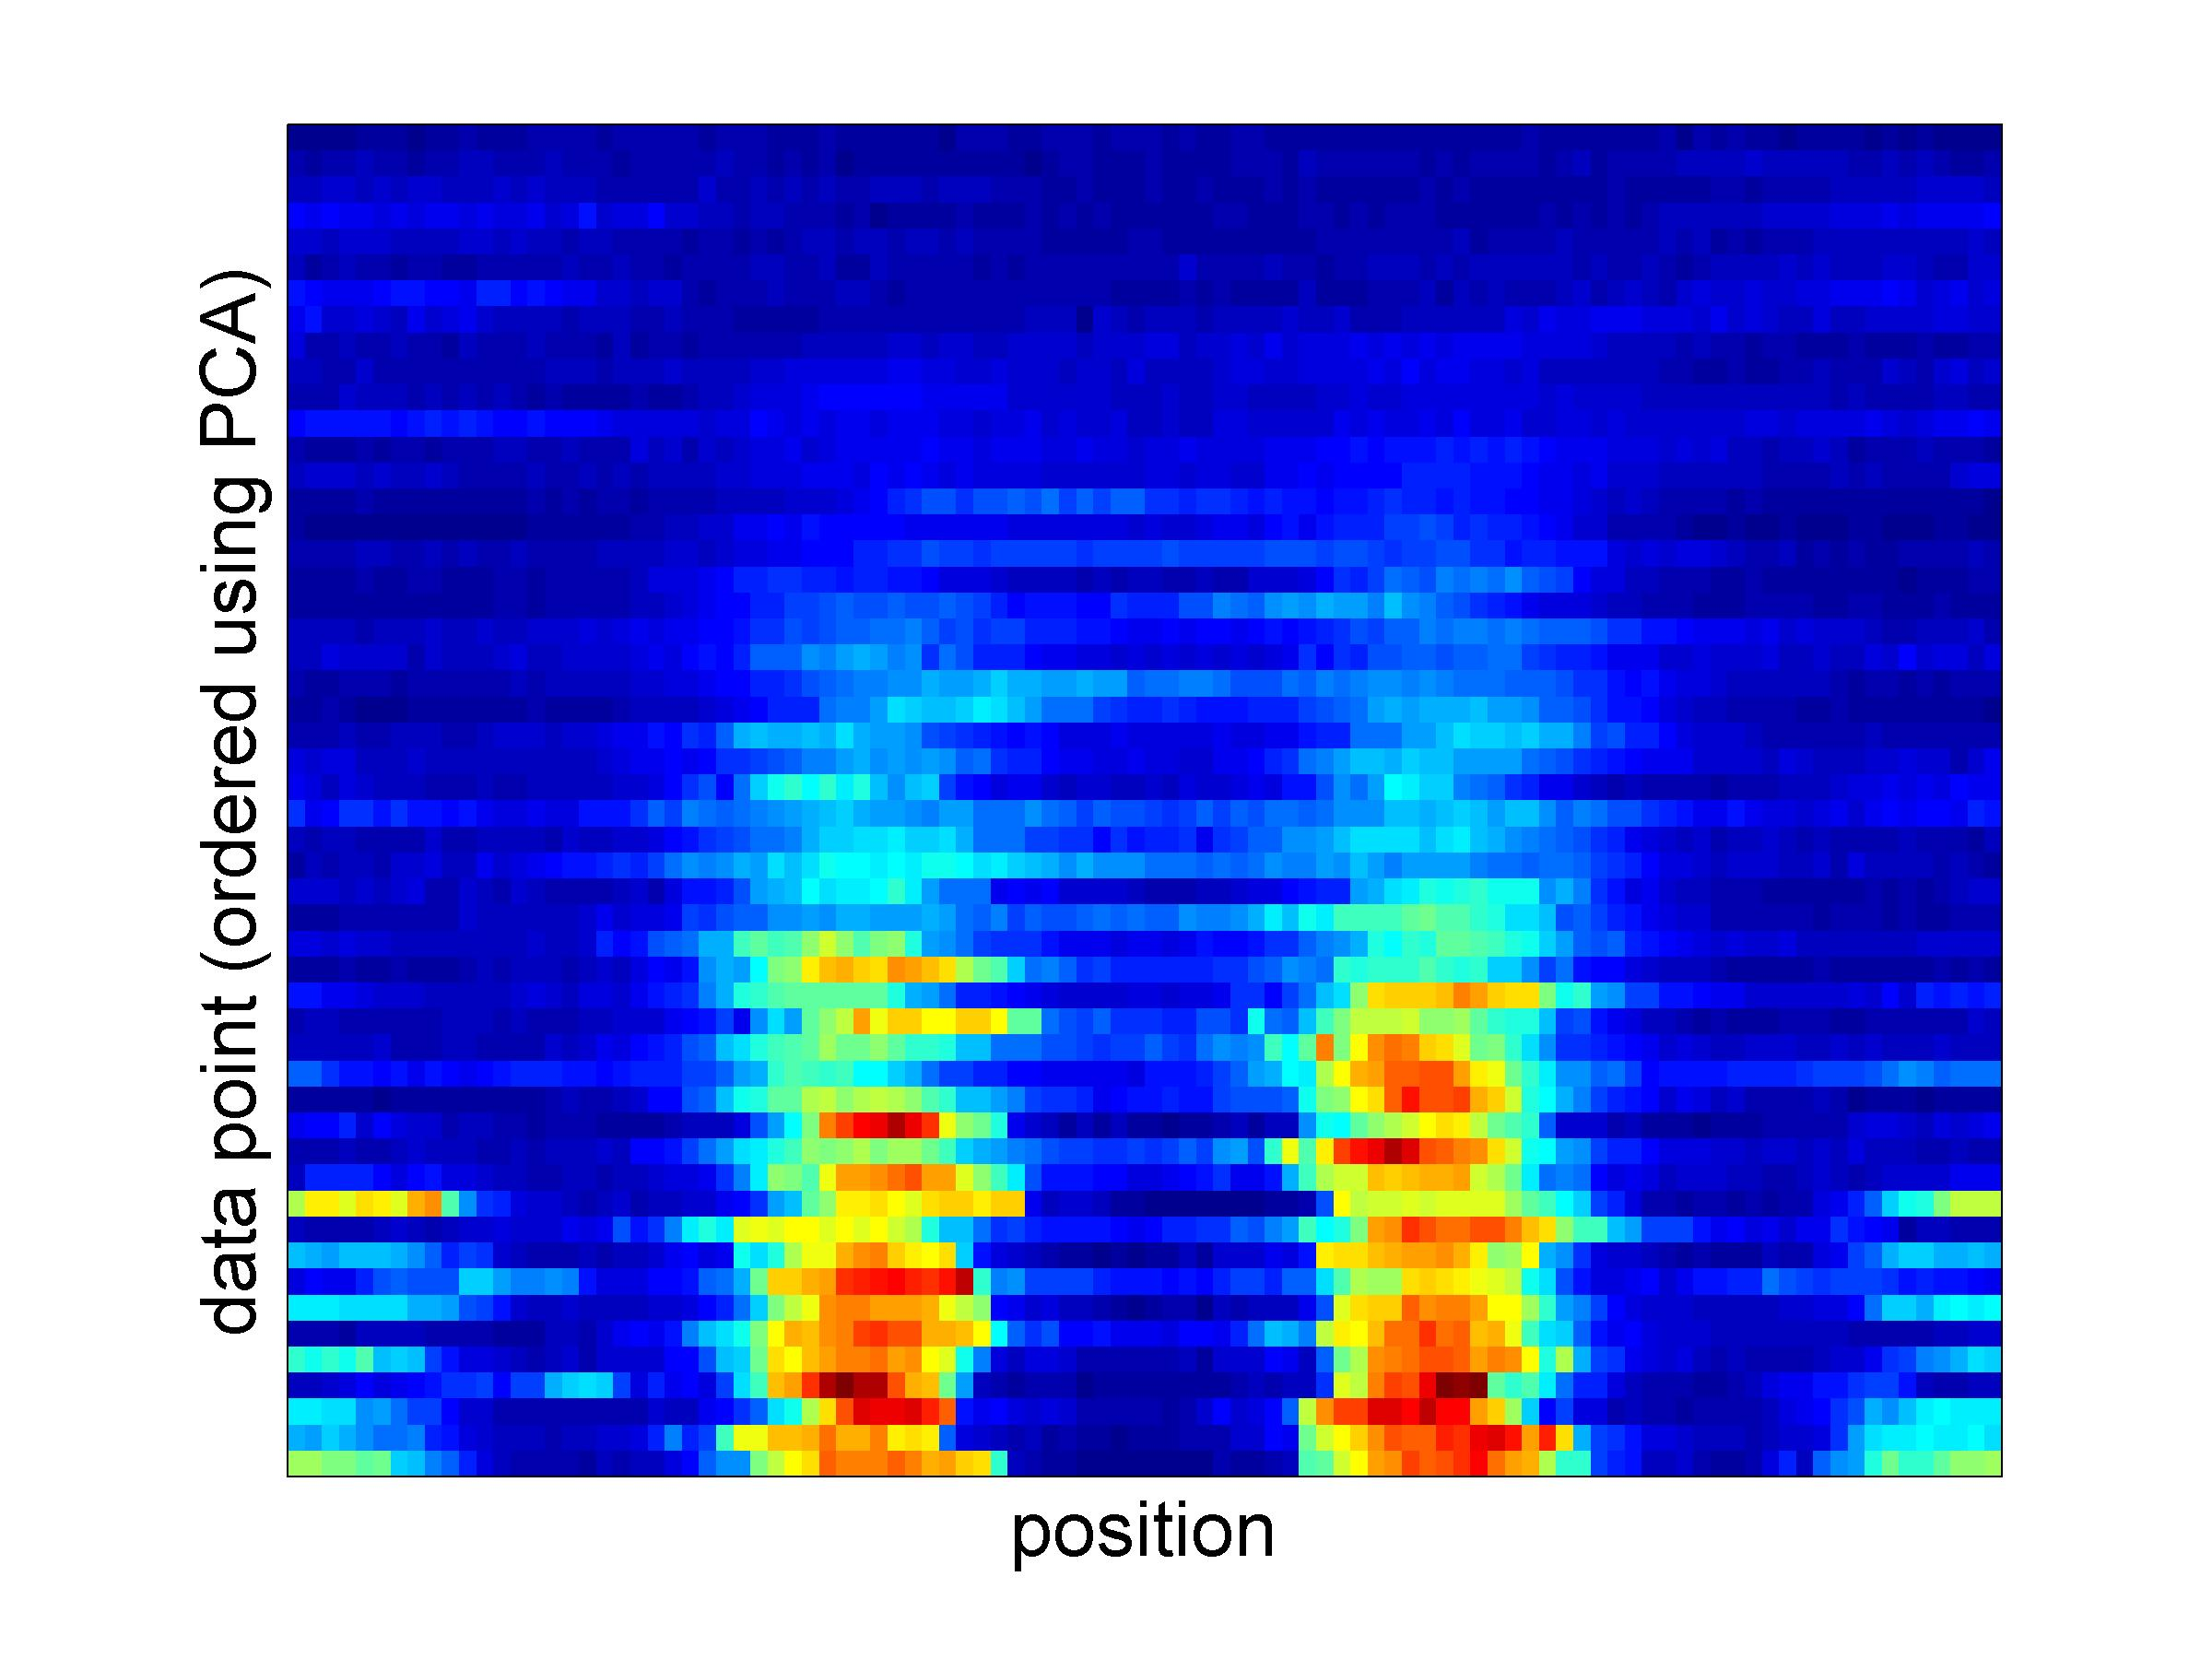
\includegraphics[width=0.5\textwidth]{data_ordered_PCA}};
    	\begin{scope}[x={(PCA_fig.south east)},y={(PCA_fig.north west)}]
    	%\draw[help lines,xstep=.05,ystep=.05] (0,0) grid (1,1);
    	\draw[rounded corners=1mm, line width=0.5mm, red] (0.13,0.13) rectangle (0.22,0.3);
    	\draw[rounded corners=1mm, line width=0.5mm, red] (0.81,0.13) rectangle (0.9,0.3);
    	\end{scope}
    	\node[anchor=south west, right of=PCA_fig, node distance=0.5\textwidth] (DMAPS_fig) {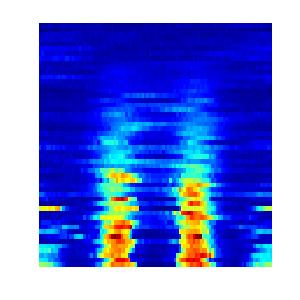
\includegraphics[width=0.5\textwidth]{data_ordered_DMAPS}};
    	\begin{scope}[shift={(DMAPS_fig.south west)},x={(DMAPS_fig.south east)},y={(DMAPS_fig.north west)}]
    	\draw[rounded corners=1mm, line width=0.5mm, red] (0.13,0.13) rectangle (0.22,0.3);
    	\draw[rounded corners=1mm, line width=0.5mm, red] (0.81,0.13) rectangle (0.9,0.3);
    	\end{scope}
    \end{tikzpicture}
    
   
    The ordering of the large central peaks is comparable.\\
    However, the outer peaks are grouped together in the right picture \\ (we could view this as ``better'').

\end{frame}

\begin{frame}{Nonlinear Orderings of Data}

	\centering
	Below are the first two projection coefficients for the data \\
	(each point corresponds to a data point/concentration profile).
	
    \centering
    \only<1>{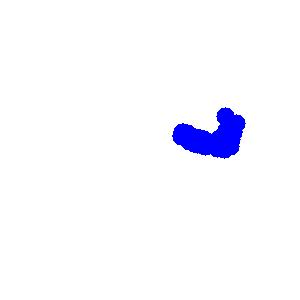
\includegraphics[width=0.6\textwidth]{coeff_12_new}}
    \only<2>{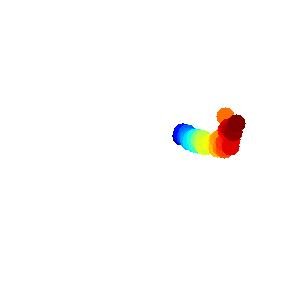
\includegraphics[width=0.6\textwidth]{coeff_12_colored}}
	
    We only use the first coefficient in the PCA ordering.
	\pause
	
	The ordering of the data produced with this coloring would perhaps be better. \\
    PCA cannot detect this ordering because it is nonlinear.
    
\end{frame}

\begin{frame}{Diffusion Maps (DMAPS) for Dimensionality Reduction}
\centering
Unlike PCA, diffusion maps \footnote{ \tiny Coifman {\em et al}, PNAS, 2005.} is a {\em nonlinear} dimensionality reduction technique

	\begin{columns}
	\begin{column}{0.4\textwidth}
		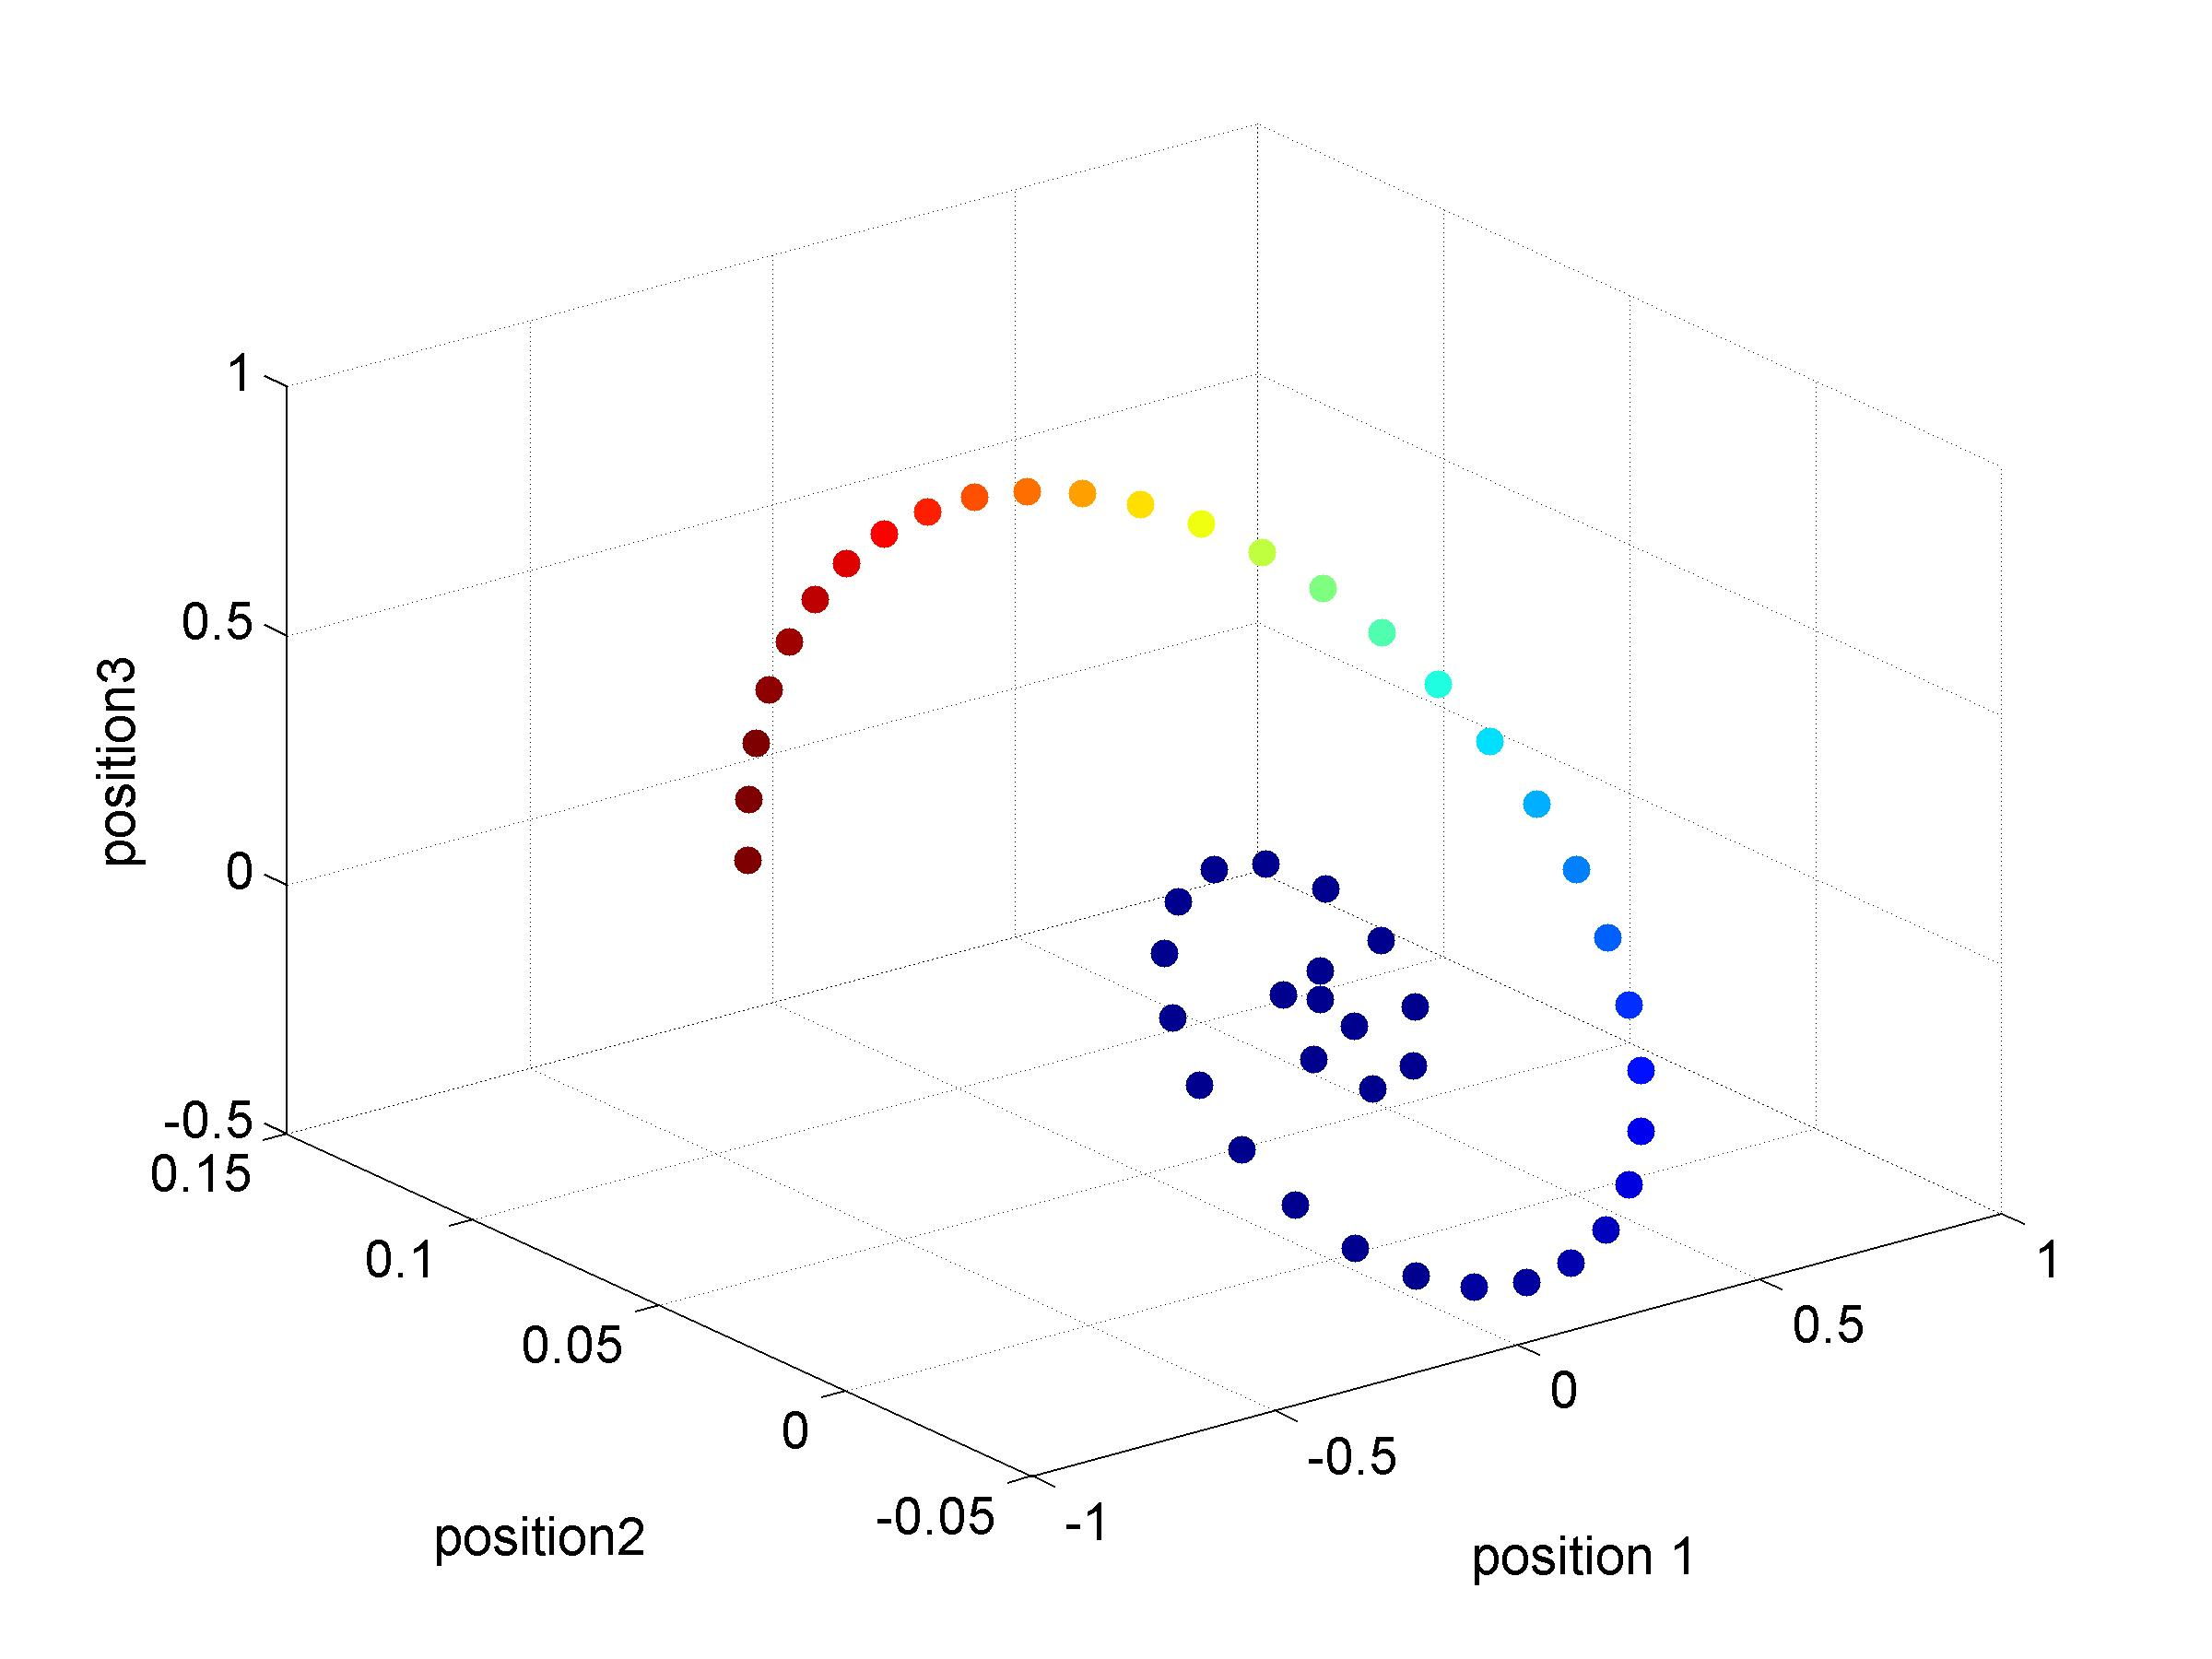
\includegraphics[width=\textwidth]{../Stas_data/group_meeting_5Feb2013/dmaps_spiral.jpg}
	\end{column}
	\begin{column}{0.5\textwidth}
	\begin{block}{DMAPS Algorithm}
		{\scriptsize 
		Calculate weight matrix $W$ with
		$$W_{ij} = exp\left( -\frac{d^2(x_i, x_j)}{\epsilon} \right)$$
		Calculate diagonal matrix $D$ with $D_{ii} = \sum_j W_{ij}$
		
		The embedding coordinates are given by the {\bf top~eigenvectors} of $D^{-1}W$
		\par}
	\end{block}
	\end{column}
	\end{columns}
%On the left you see data that has been ordered and colored using PCA.
%On the right you see data that has been ordered and colored using DMAPS.

\vspace{0.2in}

The spiral has been colored using DMAPS.

PCA would not be able to order the data on the right ``correctly'', \\since the curve is one-dimensional, but non-linear.

\end{frame}

\begin{frame}{Using DMAPS to Order Concentration Profiles}

	
	\centering
	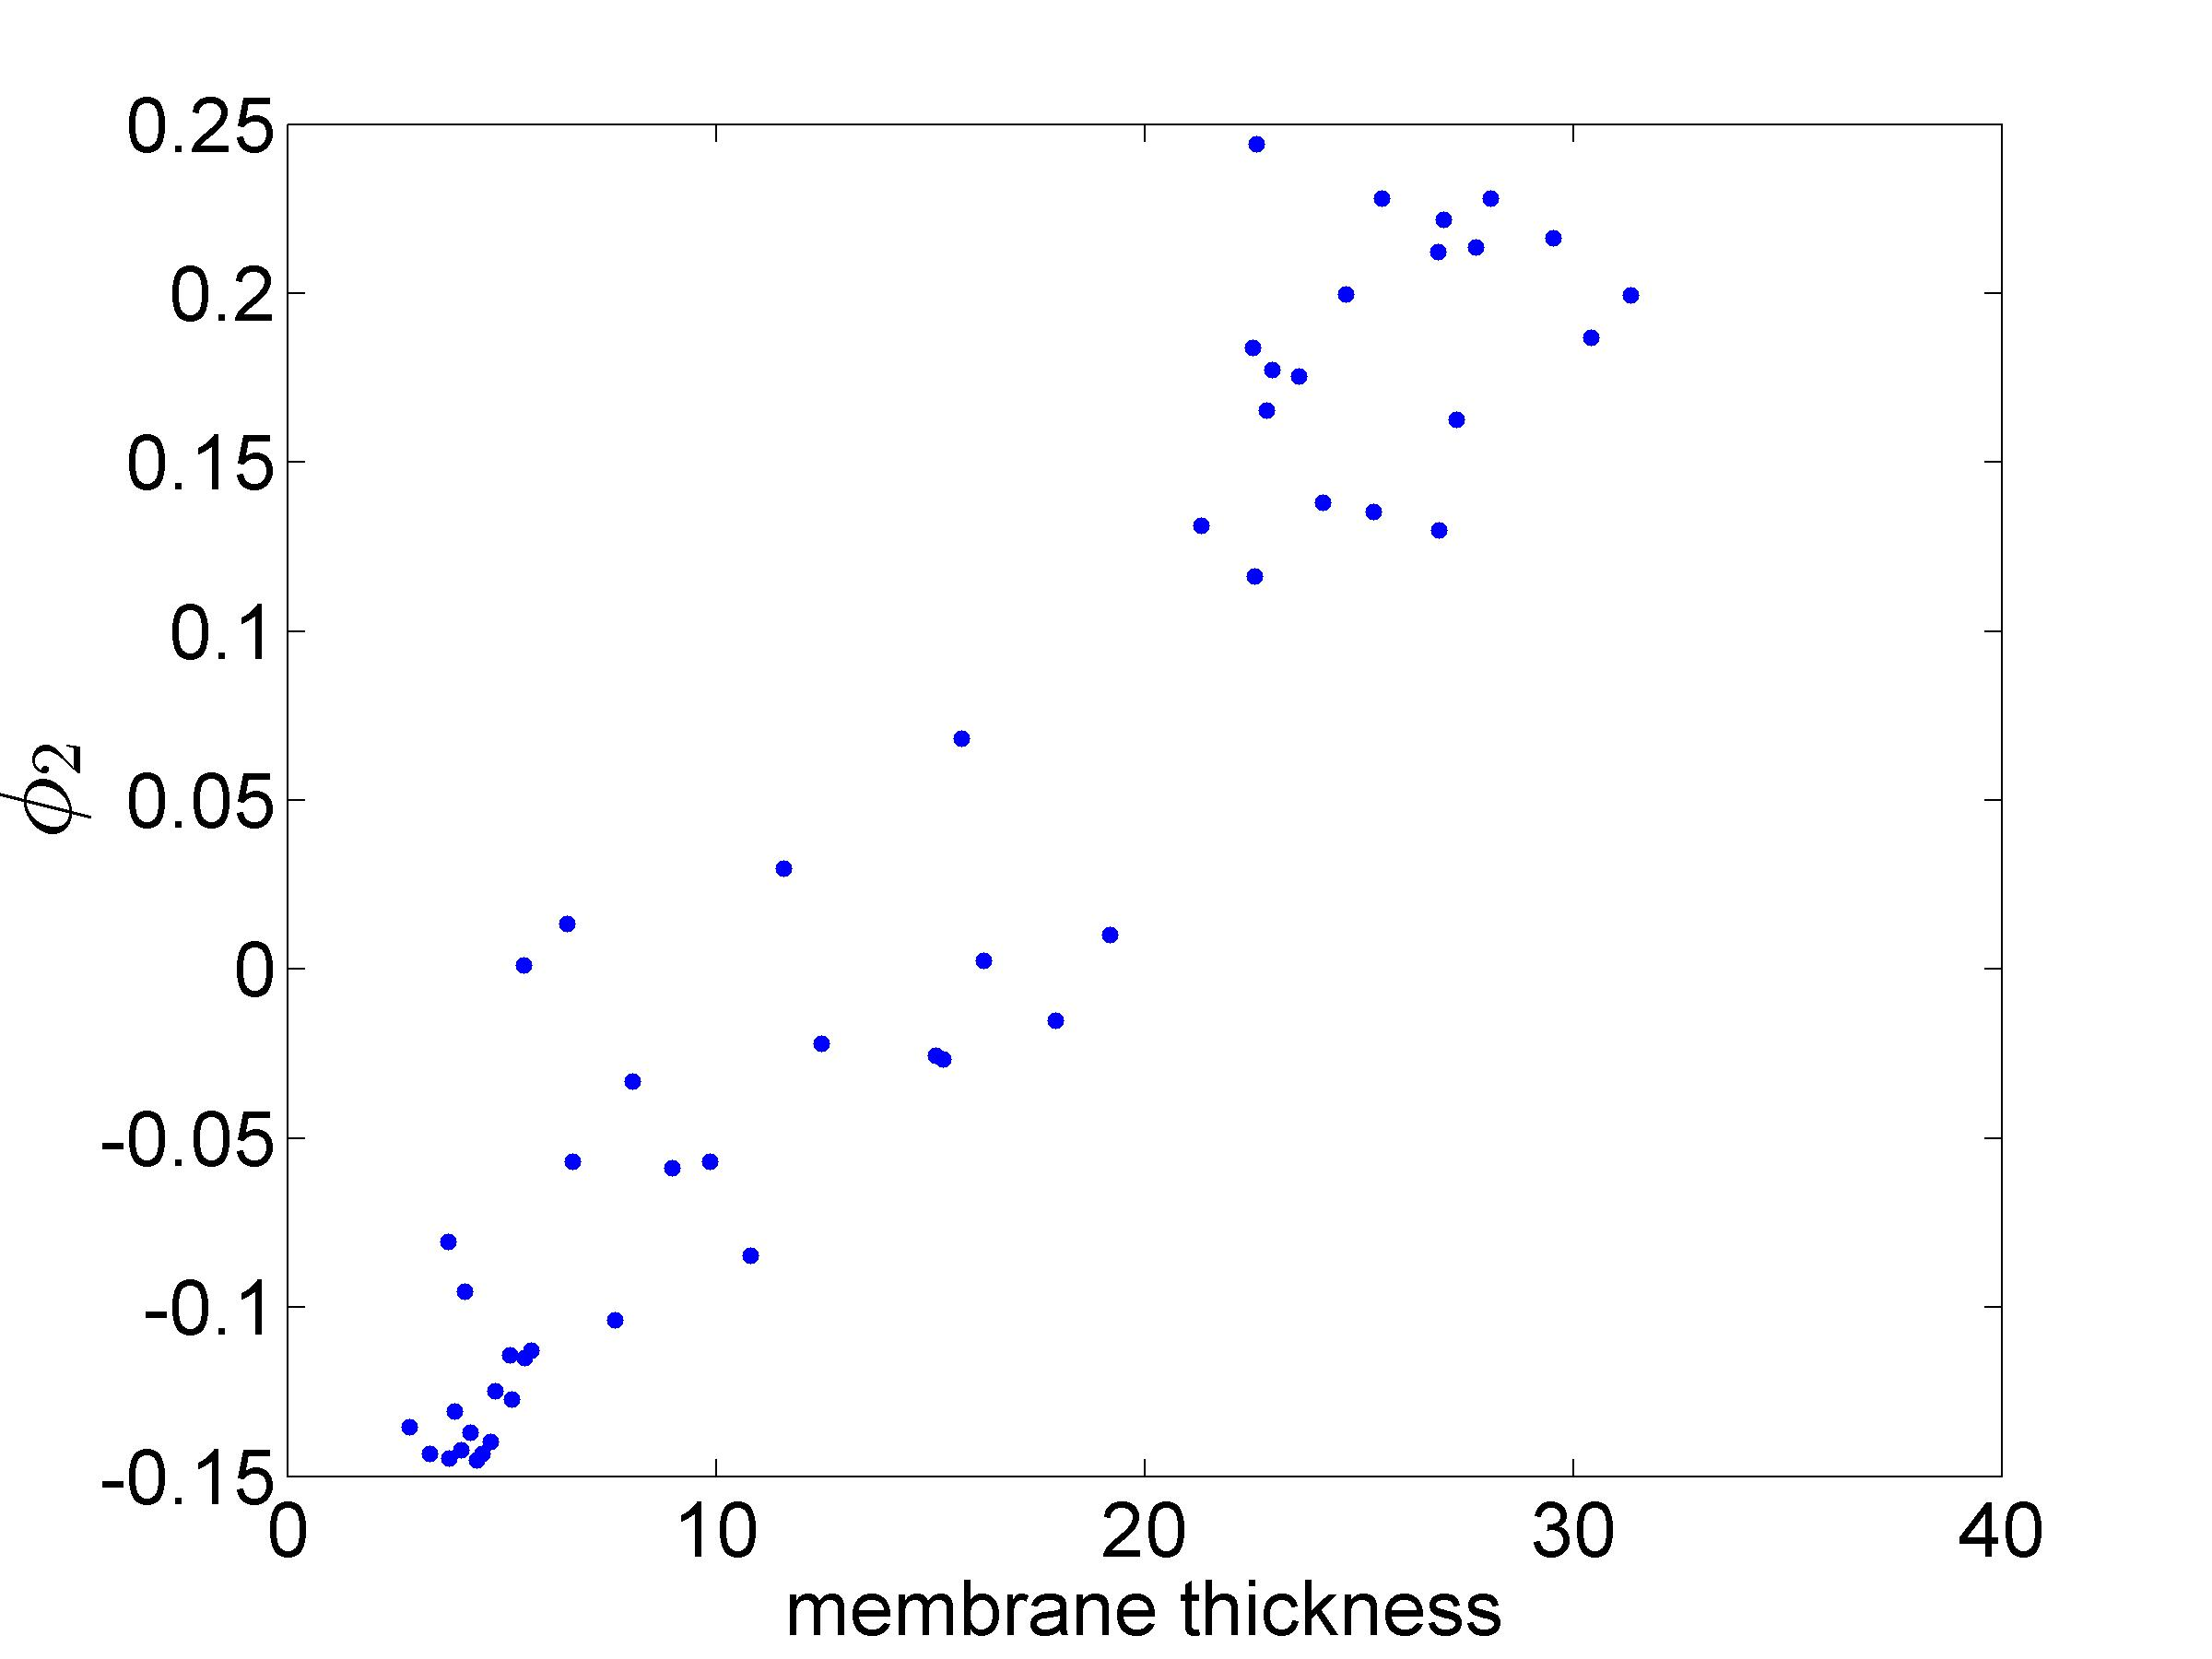
\includegraphics[width=0.3\textwidth]{DMAPS_time_corr}	
	
	\centering
  \begin{tikzpicture}
  	\node (unordered) {\includegraphics[width=0.3\textwidth]{data_unordered}};
  	\node[right of=unordered, node distance=0.5\textwidth] (ordered) {\includegraphics[width=0.3\textwidth]{data_ordered_DMAPS}};
    \draw [->] (unordered.east) -- (ordered.west);    
  \end{tikzpicture}
  
  There is a significantly better grouping of the secondary peaks when using DMAPS.
\end{frame}

\section[Factoring Out Symmetries in Concentration Profiles]{Factoring Out Symmetries in Concentration Profiles}

\begin{frame}{Importance of Symmetries in Data Analysis}

	\centering
	In the previous analysis, we first needed to determine \\where to open and ``unroll'' the circle to obtain a linear profile.
	
	\centering
	\begin{tikzpicture}
		\node (drosophila_line) {\includegraphics[width=0.2\textwidth]{circle_profile}};
		\node[right=0.3\textwidth of drosophila_line] (drosophila_circle) {\includegraphics[width=0.25\textwidth, height=0.1in]{line_profile}};
		\draw[->] (drosophila_line) -- (drosophila_circle) node[above,midway] {``Unroll'' circle};
	\end{tikzpicture}
	
	This is done by staining for {\em another} protein (Dorsal) that is expressed only along the ventral midline, and opening each profile at its dorsal midline. 
	
	\vspace{0.2in}
	
	Instead, we would like to work {\em directly} with the circular concentration profiles, and align the concentration profiles {\em automatically}, without staining for a second protein. 

\end{frame}

%\begin{frame}{How to Address Rotation Invariance in Data Analysis}
%    There are two ways to view rotation-invariant data
% 
% 	\begin{block}{}
%        \begin{tikzpicture}
%        	\node[text width=0.3\textwidth] (text1) {{\bf We can use rotations to {\em augment} data} \\ Given a data point $x$, we include all rotations of $x$ in our data set \par};
%            \node[right=of text1] (fig1) {\includegraphics[width=0.25\textwidth]{drosophila_rot1.jpg}};
%            \node [right of=fig1, node distance=0.35\textwidth] (fig2) {
%            \begin{minipage}{0.25\textwidth}
%                \includegraphics[width=0.45\textwidth]{drosophila_rot1.jpg}
%                \includegraphics[width=0.45\textwidth]{drosophila_rot3.jpg}\\
%                \includegraphics[width=0.45\textwidth]{drosophila_rot5.jpg}
%                \includegraphics[width=0.45\textwidth]{drosophila_rot7.jpg}
%            \end{minipage}};
%            \draw [->] (fig1.east) -- (fig2.west);
%        \end{tikzpicture}
%        {\scriptsize \em This results in sines and cosines as PCA modes \footnotemark \par}
%	\end{block}
%	
%	\footcitetext{sirovich1987turbulence}
%	
%	\vspace{-0.3in}
%	
%	\begin{block}{}
%        \begin{tikzpicture}
%        	\node [text width=0.3\textwidth] (text1) {{\bf We can use rotations to {\em reduce} data} \\ We first align the data before doing further analysis};
%            \node[right=of text1] (fig1) {
%            \begin{minipage}{0.25\textwidth}
%            \includegraphics[width=0.45\textwidth]{drosophila_rot1.jpg}
%            \includegraphics[width=0.45\textwidth]{drosophila_rot3.jpg}\\
%			\includegraphics[width=0.45\textwidth]{drosophila_rot5.jpg}
%            \includegraphics[width=0.45\textwidth]{drosophila_rot7.jpg}
%            \end{minipage}};
%            
%            \node [right of=fig1, node distance=0.35\textwidth] (fig2) {
%            \begin{minipage}{0.25\textwidth}
%            \includegraphics[width=0.45\textwidth]{drosophila_rot1.jpg}
%            \includegraphics[width=0.45\textwidth]{drosophila_rot1.jpg}\\
%            \includegraphics[width=0.45\textwidth]{drosophila_rot1.jpg}
%            \includegraphics[width=0.45\textwidth]{drosophila_rot1.jpg}
%            \end{minipage}};
%            \draw [->] (fig1.east) -- (fig2.west);
%        \end{tikzpicture}
%	\end{block}
%
%    We will {\bf reduce} the data by factoring out the underlying rotations
%\end{frame}

\begin{frame}{Aligning Images Under Rotations}
	
	\begin{itemize}
	\item We assume that we have many {\em rotated} copies of an image.
	%
	\item We would like to align the images so that we can perform further analysis that will be {\em invariant} to rotations. 
	%
	\item This is essential for our {\em Drosophila} data, because the developmental dynamics are invariant to the orientation of the embryos in the microfluidic device.
	\end{itemize}

	\centering
	\includegraphics[width=0.5\textwidth]{PU_clean}\\
	{\scriptsize Many rotated copies of the Princeton University shield. We will use this to illustrate how different alignment algorithms perform. }	

\end{frame}

\begin{frame}{Template-Based Alignment}
	\centering	
	
	If we have many images and wish to align them, \\ we can rotate each one until it is optimally aligned with a {\bf template}.

	In this case, we have chosen the template to be one of the images in the dataset.

	\only<1>{\includegraphics[width=0.6\textwidth]{PU_template1_clean}\\
	{\small \em Images, unaligned. The template is shown in the center. }}
	\only<2>{\includegraphics[width=0.6\textwidth]{PU_template2_clean}\\
	{\small \em Images, aligned to template. The template is shown in the center.}}
		
\end{frame}

\begin{frame}{Template-Based Alignment Under Noisy Conditions}

	\centering
	However, if the images are noisy, 
	\\then template-based alignment will often be inaccurate.

	\only<1>{\includegraphics[width=0.6\textwidth]{PU_template1_noisy}\\
	{\small \em Images, unaligned, now corrupted with white Gaussian noise. The template is shown in the center.}}
	\only<2>{\includegraphics[width=0.6\textwidth]{PU_template2_noisy}\\
	{\small \em Images, aligned to template. The template is shown in the center.}}
	\only<3>{\includegraphics[width=0.6\textwidth]{PU_template3_noisy}\\
	{\small \em Images, denoised after being aligned to template. The template is shown in the center. Note that there are several misalignments. }}
	
\end{frame}

\begin{frame}{Angular Synchronization for Alignment}
	
	Instead, we would like to use each image as a template for every other image, and then find the most {\em consistent} set of alignments. This is called {\bf angular synchronization}.
	
	\begin{minipage}{0.55\textwidth}	
	\centering
	\only<1>{\includegraphics[width=\textwidth]{PU_angsynch1} \\
	{\small \em Images, unaligned, now corrupted with white Gaussian noise.}}
	\only<2>{\includegraphics[width=\textwidth]{PU_angsynch2}\\
	{\small \em Images, aligned using angular synchronization.}}
	\only<3>{\includegraphics[width=\textwidth]{PU_angsynch3} \\
	{\small \em Images, aligned using angular synchronization and then denoised. Note that there are many fewer misalignments.}}
	\end{minipage}
	%
	\begin{minipage}{0.4\textwidth}
	\begin{itemize}
	\item Calculate angle $\theta_{ij}$ that optimally aligns image $i$ to image $j$ for every pair $i, j$
	\item Want to find angles $\theta_1, \dots, \theta_n$ such that $\theta_i -  \theta_j \approx \theta_{ij}$
	\item Also want to satisfy {\em higher-order} consistency, e.g. we not only want $\theta_i - \theta_j \approx \theta_{ij}$, but also $\theta_i - \theta_j \approx \theta_{ik} + \theta_{kj}$. 
	\end{itemize}
	\end{minipage}
	
\end{frame}

\begin{frame}{Angular Synchronization for Data Alignment}

	\begin{block}{Angular Synchronization Algorithm \footnotemark}
		{\scriptsize 
		 We have {\bf data} $x_1, x_2, \dots, x_n$ (e.g., $x_i$ is the concentration profile of dpERK on a ring).
        
        $\theta_{ij}$ denotes the {\bf angle of rotation} that best aligns $x_i$ and $x_j$.

        We {\bf construct the matrix} $H$, where $H_{ij} = e^{i \theta_{ij}}$.

		The entries of $v_1$, the {\bf top eigenvector} of $H$, contain estimates of the optimal rotations for each data point.

		The optimal rotations $\hat{\theta_1}, \dots, \hat{\theta_n}$ are given by $e^{i \hat{\theta_i}} = \frac{v_1(i)}{|v_1(i)|}$.
		\par}
	\end{block}	
	\footcitetext{singer2011angular}
	
	We can use angular synchronization to align the concentration profiles
	
	\begin{tikzpicture}
		\node[] (fig1) {\includegraphics[width=0.25\textwidth]{data_unaligned_unordered}};
		\node[right of=fig1, node distance=0.35\textwidth] (fig2) {\includegraphics[width=0.25\textwidth]{data_aligned_unordered}};
		\node[right of=fig2, node distance=0.35\textwidth] (fig3) {\includegraphics[width=0.25\textwidth]{data_ordered_angsynch}};
		\draw[->] (fig1.east) -- (fig2.west);
		\draw[->] (fig2.east) -- (fig3.west);
		\node[below of=fig1, node distance=0.7in, text width=0.3\textwidth]{{\scriptsize Profiles are unaligned and unordered. We are allowed to shift the profiles left and right (this corresponds to rotations of the circular profiles). \par}};
		\node[below of=fig2, node distance=0.7in, text width=0.3\textwidth]{{\scriptsize Profiles are aligned using angular synchronization but temporally unordered. \par}};
		\node[below of=fig3, node distance=0.7in, text width=0.3\textwidth]{{\scriptsize Profiles are then ordered in time using DMAPS. \par}};
	\end{tikzpicture}

\end{frame}

\begin{frame}{Vector Diffusion Maps: Synchronization and DMAPS}
	Our data contains both symmetries {\em and} dynamics
	
	\begin{minipage}{0.45\textwidth}
	\begin{block}{Diffusion maps}
		Calculate top eigenvectors of $W$, where $W_{ij} = e^{-\frac{d^2(x_i, x_j)}{\epsilon}} / \sum_j e^{-\frac{d^2(x_i, x_j)}{\epsilon}} $
	\end{block}
	\end{minipage}	
	\hfill
	\begin{minipage}{0.45\textwidth}	
	\begin{block}{Angular Synchronization}
		Calculate top eigenvector of $H$, where $H_{ij} = e^{-i \theta_{ij}}$
	\end{block}
	\end{minipage}
	
	\begin{block}{Vector Diffusion Maps (VDM) \footnotemark} 
		Calculate the top eigenvectors of $S$, where $S_{ij} = W_{ij}H_{ij}$
		
		The top eigenvectors then give us the optimal rotations {\em and} the embedding coordinates for our data
	\end{block}
	\footcitetext{singer2012vector}

	\vspace{-0.2in}
	\begin{tikzpicture}
		\node[] (fig1) {\includegraphics[width=0.3\textwidth]{data_unaligned_unordered}};
		\node[right of=fig1, node distance=0.6\textwidth] (fig2) {\includegraphics[width=0.3\textwidth]{data_ordered_vdm}};
		\draw[->] (fig1.east) -- (fig2.west) node[above,midway, text width=0.3\textwidth, align=center] { Aligned {\em and} ordered using VDM};
		%\node[below of=fig1, node distance=0.7in, text width=0.4\textwidth]{{\small Profiles are unaligned and unordered \par}};
		%\node[below of=fig2, node distance=0.7in, text width=0.4\textwidth]{{\small Profiles are aligned and ordered using vector diffusion maps} \par };
	\end{tikzpicture}
	
%	\begin{minipage}{0.4\textwidth}
%	\includegraphics[width=0.9\textwidth]{VDM_time_corr}	
%	\end{minipage}
%	\begin{minipage}{0.5\textwidth}
%	The VDM embedding coordinate, which we use to ``automatically'' order our data, is well-correlated with the membrane thickness, which is known to be monotonic in time.
%	\end{minipage}

\end{frame}

\section[Factoring Out Symmetries in Two--Dimensional~Images]{Factoring Out Symmetries in Two--Dimensional~Images}

\begin{frame}{Images Instead of Concentration Profiles}
	
	\centering
    As a preprocessing step, we have to take fluorescent images of the embryo~cross-sections and convert them to concentration profiles on a ring.
    
    \centering
    \begin{tikzpicture}
        \node (dpERKimage) {\includegraphics[width=0.25\textwidth]{drosophila_dpERK}};
        		\draw[gray,<->] (dpERKimage.south west) --  (dpERKimage.south east) node[below,midway] { \tiny $100 \mu m$};

        \node[right=of dpERKimage] (dpERKprofile) {\includegraphics[width=0.25\textwidth]{circle_profile}};
        \draw[->] (dpERKimage)--(dpERKprofile);
    \end{tikzpicture}
    
    \begin{itemize}
    	\item DMAPS only requires a distance metric.
    	\item Angular synchronization only requires us to compute pairwise alignments.
    	\item Therefore, we can do the same analysis {\em directly} on~the~raw~two--dimensional~fluorescent~images.
    	\item We will factor out {\bf translations and rotations}.
    	\item We will use the Euclidean distance between the intensities of the image pixels as our distance metric.
    \end{itemize}
    
	\end{frame}

\begin{frame}{Ordering Fluorescent Images Using Vector Diffusion Maps}

	\centering
    We align and order the images using vector diffusion maps.
    \vspace{0.1in}

	\drawunordered
    
    \drawdownarrow
    	
    \begin{minipage}{0.8\textwidth}
    \centering
	{\scriptsize {\bf VDM} \\Pairwise alignments account for translations and rotations of images \\ Euclidean distance between image pixels as metric \par}
    \end{minipage}
    
    \drawdownarrow
    
    \draworderedvdm
    
\end{frame}

\begin{frame}{Scattering Transform as Image Features}

{\small 
\begin{itemize}
	\item Thus far, we have focused on {\em aligning} the images so that we can factor out the~relevant symmetries before doing further analysis. 
	%
	\item Another option is to use {\em features} of the images that are invariant to translations and rotations, and use distances between these features in our DMAPS calculations.
	%
	\item 
	We will use the scattering transform \footcite{bruna2012invariant} as features of our images.
\end{itemize}
\par}
\vspace{-0.15in}
\begin{minipage}{0.55\textwidth}
\begin{block}{{\small Scattering transform is like the Fourier transform \par}}
\centering 
\includegraphics[width=0.75\textwidth]{scat_images/shapeimage_2}\\
{\tiny (Left) $f$ = indicator of a square, (Center) Modulus of the Fourier transform of $f$, (Right) Scattering transform of $f$ \par}
\end{block}

\vspace{-0.1in}
\begin{block}{{\small Scattering transform is robust to deformations \par}}
\centering
\animategraphics[width=0.8\textwidth,autoplay,loop]{5}{scat_images/animate_}{0}{3} 

{\tiny (Left) $f$ = Gabor atom of varying frequency and direction, (Center) Modulus of the Fourier transform of $f$, (Right) Scattering transform of $f$ \par}
\end{block}

\end{minipage}
\hfill
\begin{minipage}{0.4\textwidth}
\begin{block}{{\small Scattering transform can discriminate higher-order structures \par}}
\includegraphics[height=0.15\textheight]{scat_images/texture8-1}
\includegraphics[height=0.15\textheight]{scat_images/texture8-f1}
\includegraphics[height=0.15\textheight]{scat_images/shapeimage_3}

\includegraphics[height=0.15\textheight]{scat_images/texture8-eq}
\includegraphics[height=0.15\textheight]{scat_images/texture8-f1eq}
\includegraphics[height=0.15\textheight]{scat_images/shapeimage_4}\\
{\tiny (Left) $X_1, X_2$ = Two realizations of stationary textures. $X_2$ is obtained by equalizing random white noise according to the spectrum of $X_1$. (Center) Power spectrum of $X_1$, $X_2$. (Right) Scattering transform of $X_1$, $X_2$. High order scattering coefficients discriminate between the Gaussian process $X_2$ and the non-Gaussian $X_1$. \par}
\end{block}

\end{minipage}

\end{frame}

\begin{frame}{Ordering of Two-Dimensional Images}

	{\small 
	\begin{itemize}
		\item We compute the scattering transform coefficients \footcite{scatnet} for each image in our data set.
		\item We use the Euclidean distance {\em between the scattering transform coefficents} in~our~DMAPS calculation.
	\end{itemize}
    \par}
	
	\drawunordered
    
    	\drawdownarrow 
    	
    \begin{minipage}{0.5\textwidth}
    \centering
	{\scriptsize Scattering transform + DMAPS \par}
    \end{minipage}\\
    \drawdownarrow
    
	\draworderedscat 
    
\end{frame}

    
    

    

%%\section[Unaligned Membrane Images]{Factoring Out Symmetries in Two--Dimensional~Membrane~Images Using~Angular~Synchronization}

\begin{frame}{Validating Our Results: Comparing to Membrane Thickness}

\begin{itemize}
\item We still need to validate that our assumption about our data being effectively one--dimensional and monotonic in time.
%
\item During nuclear cycle 14, the membrane grows inward.
%
\item This membrane thickness is also monotonic in time \footcite{lim2013kinetics, lecuit2002slam}. 
\end{itemize}

    \vspace{0.1in}
    \begin{tikzpicture}
        \node (dpERK_5min) {\includegraphics[width=0.1\textwidth]{dpERK_5min}};
        \node[right=0in of dpERK_5min] (mem_5min) {\includegraphics[width=0.1\textwidth]{membrane_5min}};
        \node[below=0.1in of dpERK_5min] (dpERK_20min) {\includegraphics[width=0.1\textwidth]{dpERK_20min}};
        \node[right=0in of dpERK_20min] (mem_20min) {\includegraphics[width=0.1\textwidth]{membrane_20min}};
        \node[below=0.1in of dpERK_20min] (dpERK_45min) {\includegraphics[width=0.1\textwidth]{dpERK_45min}};
        \node[right=0in of dpERK_45min] (mem_45min) {\includegraphics[width=0.1\textwidth]{membrane_45min}};
        \node[below=0.25in of $(dpERK_45min)!0.5!(mem_45min)$, text width=0.3\textwidth, align=center](text1) {{\small \em We stain each embryo for dpERK and membrane proteins \par}};
        \node[right=0.5in of mem_20min] (calibration) {\includegraphics[width=0.3\textwidth]{calibration_curve}} edge[<-] (mem_5min) edge[<-] (mem_20min) edge[<-] (mem_45min);
        \node[below=0in of calibration, text width=0.3\textwidth, align=center](text2) {{\small \em The membrane thickness or ``furrow length'' is monotonic in time or age of the embryo \par}};
        \node[right=2.5in of mem_20min] (time_20) {20 minutes} edge[<-] (calibration);
        \node[right=2.5in of mem_5min] (time_5) {5 minutes} edge[<-] (calibration);
        \node[right=2.5in of mem_45min] (time_45) {45 minutes} edge[<-] (calibration);
        \node[below=0in of time_45, text width=0.25\textwidth, align=center](text2) {{\small \em We can calculate the age of each embryo from the membrane thickness \par}};
    \end{tikzpicture}

We can therefore assess the quality of our orderings by plotting the embedding coordinate as a function of membrane thickness; this should be one--to--one.
\end{frame}


\begin{frame}{Comparing Scattering Transform Ordering to Membrane Thickness}

	\includegraphics[width=0.5\textwidth]{DMAPS_scat_time_corr}

	The DMAPS embedding coordinate using the scattering transform (which we use to order the data) is well--correlated with the membrane thickness (which is known to be monotonic in time).
	
\end{frame}

\begin{frame}{Ordering Two--Dimensional Membrane Images}

We could also use our techniques (e.g. scattering transform + DMAPS) to temporally order the fluorescent {\em membrane} images.

\foreach \i in {15, 19, 30, 42, 45, 10, 36, 46, 47, 51, 27, 24, 28, 48, 38, 52, 34, 20, 50, 17, 6, 22, 16, 39, 33, 21, 2, 41, 9, 29, 14, 4, 8, 35, 31, 3, 40, 44, 13, 7, 18, 32, 11, 43, 25, 49, 5, 26, 23, 37, 12} {	
	\includegraphics[width=0.05\textwidth]{membrane_scat_raw_all_\i}} 
    
    	\centering
    {\Large $\downarrow$}
    
	\foreach \i in {15, 19, 30, 42, 45, 10, 36, 46, 47, 51, 27, 24, 28, 48, 38, 52, 34, 20, 50, 17, 6, 22, 16, 39, 33, 21, 2, 41, 9, 29, 14, 4, 8, 35, 31, 3, 40, 44, 13, 7, 18, 32, 11, 43, 25, 49, 5, 26, 23, 37, 12} {	
	\includegraphics[width=0.05\textwidth]{membrane_scat_all_\i}}  
	
	Because we are interested only in the membrane thickness, we first apply an edge--detection filter to the images.
	
	\end{frame}

\begin{frame}{Ordering of Two-Dimensional Membrane Images}
	
%	{\small
%	\begin{itemize}
%		\item 	We can also use the scattering transform coefficient with DMAPS to order the membrane images themselves.   
%		\item Because we are interested in the membrane thickness, we first run an edge detection algorithm \footcite{canny1986computational} to extract the membrane edges from the images.
%		\item We then use the Euclidean distance between the scattering transform coefficients of the edge detected images in a DMAPS calculation
%	\end{itemize}
%	\par}

%    \centering
%    \begin{tikzpicture}
%    	\node[anchor=south west] (image) {\includegraphics[width=0.4\textwidth]{DMAPS_membrane_scat_time_corr2}};
%    	\begin{scope}[x={(image.south east)},y={(image.north west)}]
%    	%\draw[help lines,xstep=.05,ystep=.05] (0,0) grid (1,1);
%    	\node(x1) at (0.23,0.23) {};
%    	\node(x2) at (0.50,0.38) {};
%    	\node(x3) at (0.57,0.51) {};
%    	\node(x4) at (0.61,0.62) {};
%    	\node(x5) at (0.64,0.74) {};
%    	\end{scope}
%    	\node[below=0.2in of image](fig3) {\includegraphics[width=0.1\textwidth]{membrane_scat_3}};		
%    	\node[left=0.1in of fig3](fig2) {\includegraphics[width=0.1\textwidth]{membrane_scat_2}};
%    	\node[left=0.1in of fig2](fig1) {\includegraphics[width=0.1\textwidth]{membrane_scat_1}};	
%    	\node[right=0.1in of fig3](fig4) {\includegraphics[width=0.1\textwidth]{membrane_scat_4}};					
%    	\node[right=0.1in of fig4](fig5) {\includegraphics[width=0.1\textwidth]{membrane_scat_5}};
%    	\node[below=0.02in of fig3](fig3b) {\includegraphics[width=0.1\textwidth]{membrane_scat_raw_3}};		
%    	\node[left=0.1in of fig3b](fig2b) {\includegraphics[width=0.1\textwidth]{membrane_scat_raw_2}};
%    	\node[left=0.1in of fig2b](fig1b) {\includegraphics[width=0.1\textwidth]{membrane_scat_raw_1}};	
%    	\node[right=0.1in of fig3b](fig4b) {\includegraphics[width=0.1\textwidth]{membrane_scat_raw_4}};					
%    	\node[right=0.1in of fig4b](fig5b) {\includegraphics[width=0.1\textwidth]{membrane_scat_raw_5}};	    
%    	\draw[->] (x1) -- (fig1.north);
%    	\draw[->] (x2) -- (fig2.north);
%    	\draw[->] (x3) -- (fig3.north);
%    	\draw[->] (x4) -- (fig4.north);
%    	\draw[->] (x5) -- (fig5.north);
%    \end{tikzpicture}
%    
%    The first DMAPS coordinate is well-correlated with the membrane thickness.	
    
We then compute the scattering transform of the (edge--detected) images, and use this in a DMAPS calculation.

    \foreach \i in {15, 19, 30, 42, 45, 10, 36, 46, 47, 51, 27, 24, 28, 48, 38, 52, 34, 20, 50, 17, 6, 22, 16, 39, 33, 21, 2, 41, 9, 29, 14, 4, 8, 35, 31, 3, 40, 44, 13, 7, 18, 32, 11, 43, 25, 49, 5, 26, 23, 37, 12} {	
	\includegraphics[width=0.05\textwidth]{membrane_scat_all_\i}} 
    
    	\centering
    {\Large $\downarrow$}
    
	\foreach \i in {2,...,52} {
	\includegraphics[width=0.05\textwidth]{membrane_scat_all_\i}
	}   


\end{frame}

    
    

    

\section{Conclusions}

\begin{frame}{Conclusions and Acknowledgments}
    \begin{itemize}
        \item Dimensionality reduction techniques, such as DMAPS, can help us temporally order data and reconstruct dynamics.
        \item Factoring out symmetries is essential to uncovering the underlying (symmetry-invariant) dynamics.
        \item We can work with the two-dimensional images, rather than pre--processed concentration profiles, to obtain a similar picture of developmental dynamics.
        \item These techniques are very general and can be applied to a variety of systems where longitudinal data is expensive or even impossible to collect.
        \item The essential assumption in our analysis is that the data are effectively one--dimensional and monotonic in time. 
    \end{itemize}
    
     \vfill
    
    \centering
    %\begin{minipage}{0.3\textwidth}
    	%\centering
    	%\includegraphics[width=\textwidth]{DOE_logo.png}\\
	%	{\footnotesize DE-FG02-10ER26024, \\Award Number DE-SC000517 \\ DE-FG02-09ER25877, \\Award Number DE-SC0002097 \par}
    %\end{minipage}
    \begin{minipage}{0.3\textwidth}
    	\centering
    	\includegraphics[width=0.5\textwidth]{nsf1.jpg}\\
		{\footnotesize CMMI-1310173}
    \end{minipage}
    \hfill
    \begin{minipage}{0.3\textwidth}
	    \centering
    	\includegraphics[width=\textwidth]{CSGF_horiz_1200x360.png}
    \end{minipage}
    
\end{frame}

\begin{frame}{Final Thoughts: Baer's Law and Developmental Dynamics}

\begin{minipage}{0.3\textwidth}
\centering
\includegraphics[width=\textwidth]{vonbaer} \\
Karl Ernst von Baer, 1792-1876
\end{minipage}
\hfill
\begin{minipage}{0.65\textwidth}
\centering
\includegraphics[width=\textwidth]{stages_development}\\
Embryo drawings, 1892
\end{minipage}

\end{frame}


\end{document}
